\documentclass[
print,
  11pt,
  table,   
  nolof,    
  nolot,
  oneside,final
]{fithesis3}

\usepackage[resetfonts]{cmap}
\usepackage[main=czech,english]{babel}       
%% The following section sets up the metadata of the thesis.

\thesissetup{
    university    = mu,
    faculty       = fi,
    type          = mgr,
    author        = Bc. Milan Valúšek,
    gender        =m,
    advisor       = prof. RNDr. Jiří Hřebíček\, CSc.,
    title         = {Podpora výuky matematiky v~LMS Moodle s~využitím Maple T.A.},
    TeXtitle      = {Podpora výuky matematiky v~LMS Moodle s~využitím Maple T.A.},
    keywords      = {E-learning, Learning Management system, Learning Tools Interoperability, Moodle, Maple T.A., webové služby, integrace },
    TeXkeywords   = {E-learning, Learning Management system, Learning Tools Interoperability, Moodle, Maple T.A., webové služby, integrace },
}
\thesislong{abstract}{
Práce se zabývá e-learningovými systémy LMS Moodle a Maple T.A., jejich základním stavebním prvkům a použití. Dále analyzuje možnosti rozšíření systému Moodle a existující možnosti integrace se systémem Maple T.A. V~poslední části práce je navržen a implementován vlastní způsob integrace.
}
\thesislong{thanks}{
Rád bych poděkoval vedoucímu práce panu prof. RNDr. Jiřímu Hřebíčkovi, CSc. za jeho
odborné vedení a pomoc při přípravě této práce. Dále bych rád poděkoval svým rodičům a blízkým za podporu během celého studia. 
}
%% The following section sets up the bibliography.
\usepackage{csquotes}
\usepackage[              %% When typesetting the bibliography, the
  backend=biber,          %% `numeric` style will be used for the
  style=numeric,          %% entries and the `numeric-comp` style
  citestyle=numeric-comp, %% for the references to the entries. The
  sorting=none,           %% entries will be sorted in cite order.
  sortlocale=auto         %% For more unformation about the available
]{biblatex}               %% `style`s and `citestyles`, see:
%% <http://mirrors.ctan.org/macros/latex/contrib/biblatex/doc/biblatex.pdf>.
\addbibresource{my_bib.bib} %% The bibliograpic database within
                          %% the file `example.bib` will be used.
\usepackage{makeidx}      %% The `makeidx` package contains
              %% helper commands for index typesetting.
%% These additional packages are used within the document:
\usepackage{paralist}
\usepackage{amsmath}
\usepackage{amsthm}
\usepackage{amsfonts}
\usepackage{url}
\usepackage{breakurl} 
\usepackage[breaklinks]{hyperref}
\usepackage{menukeys}
\usepackage{ragged2e}  % for '\RaggedRight' macro (allows hyphenation)

\usepackage{listings}
\usepackage{color}
\newcolumntype{Y}{>{\RaggedRight\arraybackslash}X} 
\makeatletter\thesis@load
  \makeatletter
    \def\thesis@blocks@thanks{%
      \ifx\thesis@thanks\undefined\else
	\thesis@blocks@clear
	\begin{alwayssingle}%
	  \chapter*{\thesis@@{thanksTitle}}%
	  \thesis@thanks
	\end{alwayssingle}%
      \fi}
  \makeatother

\setcounter{biburllcpenalty}{7000}
\setcounter{biburlucpenalty}{8000}

\renewcommand{\lstlistingname}{Úryvek}
\renewcommand{\lstlistlistingname}{Seznam úryvků}
\definecolor{codegreen}{rgb}{0,0.6,0}
\definecolor{codegray}{rgb}{0.5,0.5,0.5}
\definecolor{codepurple}{rgb}{0.58,0,0.82}

 
\lstdefinestyle{mystyle}{
    backgroundcolor=\color{white},   
    commentstyle=\color{codegreen},
    keywordstyle=\color{magenta},
    numberstyle=\tiny\color{codegray},
    stringstyle=\color{codepurple},
    basicstyle=\footnotesize,
    breakatwhitespace=false,         
    breaklines=true,                 
    captionpos=b,                    
    keepspaces=true,                 
    numbers=left,                    
    numbersep=5pt,                  
    showspaces=false,                
    showstringspaces=false,
    showtabs=false,                  
    tabsize=2
}
 
\lstset{style=mystyle}


\begin{document}


\chapter{Úvod}


Moderní svět je již v~dnešní době závislý na moderních technologiích. Vyžaduje to stále více společnost, ve které technologie nevyužívají jen mladí a techničtí lidé, ale i méně technicky gramotní uživatelé. Skladba těchto uživatelů navíc je, především díky dostupnosti a rozšířenosti mobilních zařízení, velice rozmanitá a rozdíly v~úrovni vzdělání, věku, náboženství a ani sociálně-ekonomický aspekt již nehrají takovou roli \cite{itustats}. S~takto rozšiřující se základnou uživatelů moderních technologií roste poptávka po nových nástrojích a pokrytí existujících služeb mobilními (on-line) technologiemi, které neomezují uživatele místem, časem ani způsobem konzumace.


Mezi základní služby, které tento trend následují a jdou naproti svým uživatelům, se řadí i elektronické vzdělávání, tzv. e-learning. Nicméně osob\-ní kontakt s~vyučujícím a kolektivem studentů u~prezenčního studia zůstává stále důležitým aspektem v~procesu vzdělávání, proto v~nejbližších desetiletích e-learning klasické vzdělávání nejspíše nenahradí \cite{techvsteach}. I~přesto si distanční forma studia získala důležitou pozici právě díky výhodám, které přinášejí moderní on-line technologie, jež dokáží odbourat řadu překážek (distance, čas, produktivita atd.). S~e-learningem se také zvýšila dostupnost vzdělání pro poměrně velkou část populace, která nemůže studovat prezenčně a u~nichž je individuální časový plán nutností (důchodci, zaměstnaní ad.).

Nejsou to jen nové technologie, trendy nebo systémy, jež studenty doprovázejí v~distančním vzdělávání; jsou to především tutoři a materiály, které jsou prezentovány nástroji určenými pro vzdělávání. Na druhou stranu prezentace a možnosti nástroje hrají svou roli při přípravě materiálů, vzdělávání, koordinaci výuky, kooperaci a evaluaci studentů a jejich práce. Každý nástroj má své silné a slabé stránky. Jejich kombinací můžeme dosáhnout lepších výsledků, ale jen v~případě, že zapojení více nástrojů ve výsledku neztíží uživateli práci. Řešením jednoduchého použití více nástrojů je jejich integrace. Právě téma integrace je zajímavé a přínosné při rozvoji e-learningu, a proto je cílem této diplomové práce integrace nástroje Maple T.A. do e-learn\-ingové platformy LMS Moodle.

V~první částí diplomové práce si uvedeme definice pojmů ze světa distan\-ční výuky. Zaměříme se blíže na LMS Moodle, který patří mezi oblíbené výukové platformy, i když si s~sebou nese nálepku složitého a někdy nepřehledného softwaru, a nástroj Maple T.A., který se zaměřuje na zkoušení a testování úloh především matematického zaměření. V~rámci práce je vysvětleno, k~čemu nástroje slouží, jak se dají použít, co nabízí a jak přistupují k~uživatelům a jejich oprávněním a také jaké jsou základní stavební kameny obou systémů.

Ve druhé části práce se zaměříme na způsoby rozšíření LMS Moodle a provedeme analýzu možností integrace s~nástrojem Maple T.A. Rozebereme existující konektory a podíváme se na návrh vlastního jednoduchého řešení a detaily ze samotné implementace konektoru. Rozebereme také další možnosti rozvoje navrhovaného řešení.


\chapter{Definice pojmů}
	\section{E-learning}
E-learning se rozvíjí a mění stejně rychle jako informační technologie, které využívá, a reaguje na aktuální dění ve společnosti. Proto není divu, že se nabízí více definic pojmu e-learning. Dostatečně je pojem e-learning popsán následujícími definicemi:

\begin{enumerate}
  \item \emph{„Význam slovního spojení e-learning může být brán jako elektronic\-ké vzdělávání. Elektronické vzdělávání znamená z~hlediska učitele realizovat edukační proces elektronickými prostředky, v~současnosti přesněji informačně-komunikačními prostředky. Elektronické učení z~pozice žáka znamená realizovat těmito prostředky proces vlastního učení.“} \cite{ockajova}
  \item \emph{„E-learning je výuka s~využitím výpočetní techniky a internetu.“} \cite{korviny}
  \item \emph{„Obecně vzato představuje e-learning způsob vzdělávání, který v~yužívá moderní informační a komunikační technologie k~předávání v~ýukového obsahu, komunikaci účastníků vzdělávání a k~řízení v~ýukového procesu.” }\cite{cznic}
  \item \emph{„E-learning zahrnuje jak teorii a výzkum, tak i jakýkoliv vzdělávací proces (s~různým stupněm intencionality), v~němž jsou v~souladu s~etickými principy používány informační a komunikační technologie pracující s~daty v~elektronické podobě. Způsob využívání prostředků ICT a dostupnost učebních materiálů jsou závislé především na vzdělávacích cílech a obsahu, charakteru vzdělávacího prostředí, potřebách a možnostech všech aktérů vzdělávacího procesu.” }\cite{zounek}

\end{enumerate}


Nad rámec těchto definic můžeme e-learning také chápat jako samostudium prostřednictvím počítače, mobilu či jiného zařízení připojeného k~internetu. Materiály u~této formy výuky jsou zpravidla znovupoužitelné a jednoduše upravitelné. Nabízí učiteli téměř neomezené možnosti úprav a přístup odkudkoliv, kde má připojení k~internetu. Studentům na druhé straně nabízí často okamžitou odezvu (nejedná-li se o~úlohy vyžadující ruční úpra\-vu) a dostupnost ke studijním materiálům. Nad rámec standardních služeb nabízí také nové komunikační možnosti jako fórum, skupinový chat apod.


Na druhou stranu je potřebné podotknout, že e-learning nepřináší jen výhody. Hlavní problém, který při e-learningu nastává, je absence osobního kontaktu studenta s~učitelem a ostatními studenty, jelikož nedochází k~rozvoji dalších dovedností, jakými jsou například sebeprezentace a schopnost vyjadřovat se. Komunikace mezi učitelem a studentem navíc postrádá bezprostřední odezvu a částečně ztrácí efektivitu při řešení problému. Vedle toho přináší zvýšené nároky na učitele a jeho přípravu materiálů. Ty musí být patřičné kvality, protože podkladové materiály musí být jasné, samo-vysvětlující a zároveň by neměly být příliš obsáhlé, aby studenta nesváděly jen k~rychlé povrchní prohlídce.

Slovo e-learning se často nesprávně zaměňuje s~pojmem „on-line výuka“. Vysvětleme si tedy rozdíl mezi těmito dvěma výrazy. On-line výuka předpokládá on-line (přímé) spojení mezi učitelem a studentem. Učitel tedy musí být připojený ve stejnou chvíli jako student, aby mohl komunikovat se studentem, odpovídat na jeho dotazy, radit mu, zkoušet ho. Učitel sice může být vzdálen od studenta několik desítek kilometrů, ale musí být fyzicky přítomen u~počítače a interaktivně se studentem pracovat \cite{striteska}. Pojem „e-learn\-ing“ kromě on-line výuky zahrnuje způsob vyučování, které rovněž probíhá vzdáleně, ale nemusí existovat přímé spojení mezi vyučujícím a studentem. Není po nich vyžadována přítomnost na stejném místě, ani ve stejný čas.


	\section{Distanční vzdělávání}

Výše zmíněné definice e-learningu mají společného jmenovatele, kterým jsou informační technologie. E-learning se tak stává prostředkem tzv. distančního vzdělávání. V~následujícím textu jsou popsány jeho základní definice: 

      \begin{itemize}
	\item \emph{„Distanční vzdělávání je multimediální forma řízeného samostatné\-ho studia, které je koordinováno vzdělávací institucí a v~němž jsou vyučující resp. konzultanti (tutoři) v~průběhu vzdělávání trvale nebo převážně fyzicky odděleni od vzdělávaných. Multimediálnost zde znamená využití všech dostupných a účelných didaktických prvků a technických prostředků, kterými lze prezentovat učivo, komunikovat se studujícími, provádět průběžné hodnocení studijních pokroků a případně také hodnotit závěrečné výsledky studia. Aktuální a efektivní technologickou podporou distančního studia je metoda e-learn\-ing.“} \cite{zlamalova} 
	\item Podle \cite{prucha} se \emph{„jedná o~formu studia zprostředkovaného médii (telefon, rozhlas, televize, počítač, zvl. internet a elektronická pošta aj.). Je založeno na samostatném studiu účastníků, řízeném specializovanou institucí, bez prezenčního kontaktu studujících s~vyučujícími. Výuku účastníků zajišťují speciálně připravené učební materiály (výukové balíky) a jiné metody studijní podpory a hodnocení, umožňující individuální přístup.“} 
	\item \emph{„Zde je základem samostudium a speciálně zpracovaný obsah studia (v~podobě tištěné nebo elektronické). Obsah studia není tvořen klasickými učebnicemi nebo skripty, ale jedná se o~metodicky propracovaný materiál, který umožňuje studujícím pochopit učivo bez každodenního kontaktu s~vyučujícím. Výkony studentů jsou průběžně sledovány (např. pomocí dílčích úkolů či testů), studentům je k~dispozici učitel – tutor.“}\cite{cznic}

	\item \emph{„Distanční forma je samostudium, kdy výuka neprobíhá v~učebnách a nevyžaduje se osobní účast učitelů a studentů ve škole. Student se školou komunikuje např. prostřednictvím počítačových interaktivních programů, e-mailu, internetu, záleží na  možnostech školy, především její technické vybavenosti. Užívaným informačním technologiím jsou metodicky i didakticky přizpůsobeny veškeré učební pomůcky.“} \cite{nuov}
     \end{itemize}

Distančním vzděláváním se, nejen na základě zmíněných definic, myslí alternativní styl výuky, který nevyžaduje přímý kontakt mezi aktéry výuky. Naopak probíhá převážně formou samostudia, které je řízeno připravenými materiály, s~případnou pomocí tutora. Využívá různých komunikačních kanálů, se zvláštním zaměřením na internet a služby s~ním spojené (elektronická pošta, konference, video kanály, webové prezentace, e-learn\-ingové platformy apod.).


	\section{Learning management system}
Learning management system (zkráceně LMS) je označení jakéhokoliv balíku softwarových nástrojů sloužícího k~e-learningu, které jsou dostupné online, nejčastěji z~webového rozhraní. Hlavním, nikoliv jediným, nástrojem je tvorba, distribuce a administrace vzdělávacích kurzů a materiálů. Vedle nástroje pro správu kurzů LMS obsahuje také tyto části \cite{lms}:
\begin{itemize}
	\item Evidence a správa žáků
	\item Katalog výukových kurzů a objektů
	\item Správa studijních plánů
	\item Evidence hodnocení žáků
	\item Testování a zkoušení žáků
	\item Správa přístupových práv
	\item Komunikační nástroje
	\item Autorské nástroje k~vytváření výukových kurzů a objektů
	\item Úložiště výukového obsahu
\end{itemize}
Jednotlivá řešení LMS nemusí nutně zahrnovat všechny tyto nástroje a naopak mohou nabízet širší paletu nástrojů.

	\section{Learning Tools Interoperability}
Learning Tools Interoperability{\textregistered} (dále jen LTI) je specifikace vytvořená organizací IMS Global Learning Consortium a jejím cílem je ustanovení standardního přístupu k~integraci výukových aplikací (často poskytované jako služby třetích stran) s~výukovými platformami, jakými jsou LMS, CMS, portály, výukové repozitáře a další prostředí pro podporu výuky. V~praxi to znamená přímočarou a bezimplementační integraci nástrojů s~odlišnou funkcionalitou pomocí jednotného rozhraní, což vede ke snížení časových i finančních nákladů při integraci napříč systémy. \cite{imslti}

\begin{figure}[htb]
		  \begin{center}
		    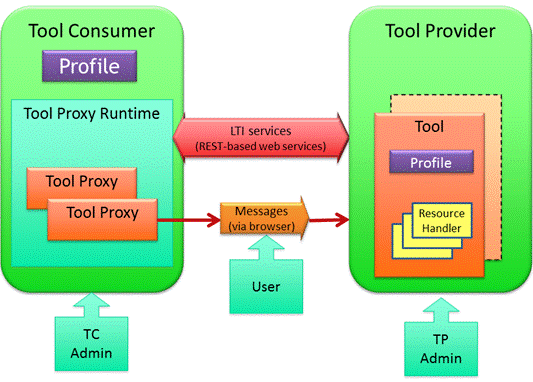
\includegraphics[width=100mm]{images/ltipic.png}
		   \end{center}
		  \caption{Koncept spolupráce mezi konzumentem a poskytovatelem. \cite{imslti20}}
		  \label{fig:ltipic}
		\end{figure}
Klíčovým konceptem LTI je „konzument” a „poskytovatel” (obrázek \ref{fig:ltipic}). Specifikace udává jednotné rozhraní mezi e-learningovým nástrojem poskytujícím služ\-by a e-learningovou platformou konzumující služby. V~praxi je typických konzumentem LMS na bázi Moodlu nebo Blackboardu\footnote{\url{http://uki.blackboard.com/}}, ale není to podmínkou, a typickým poskytovatelem je software třetích stran podobný nástrojům Wimba\footnote{\url{http://www.wimba.com/}}, Mahara e-portfolio\footnote{\url{https://mahara.org/}} nebo třeba Maple T.A.. Specifikace LTI podporuje širší definici konzumenta i poskytovatele zahrnující například studentské portály (konzumenti) a různorodé externě hostované funkcionality (poskytovatelé). \cite{imsltiinvest}


Specifikace LTI má dvě hlavní větve: LTI 1 a LTI 2, kterými lze integrovat systémy. LTI 1 bylo poprvé uvolněno v~roce 2006, kdy bylo příliš komplexní a neujalo se. Další vydání se snažila specifikaci zjednodušit. V~roce 2012 je vydána verze LTI 1.1 a později téhož roku LTI 1.1.1. Právě tyto verze se využívají pro integraci mezi systémy, poskytují základní a jednoduché rozhraní pro komunikaci a přenos informací.

LTI 2 byla dlouho vyvíjená verze, která byla vydána v~lednu roku 2015. Umožňuje přenášení více informací (aktivní přenos výsledků, více sofistikovaný přenos informací a rozšiřitelnou množinu informací pro hlubší integraci) mezi systémy v~obou směrech komunikace a přináší větší kontrolu a svobodu v~umístění odkazů na poskytující software. Vzhledem k~tomu, že se jedná o~relativně novou specifikaci, není její implementace tolik rozšířená. \cite{imslti20}


\chapter{LMS Moodle}
Cílem této kapitoly je představit LMS Moodle, jeho základní stavební kameny, práci s~kontexty, uživatelskými rolemi  a postup založení a nastavení konkrétního kurzu.

	\section{Co je to Moodle?}

Moodle je software pro tvorbu výukových systémů a elektronických kurzů na internetu. Jedná se o~neustále se vyvíjející projekt (již od roku 1999), navržený na základě sociálně konstruktivistického\footnote{Více na \url{https://docs.moodle.org/archive/cs/V\%C3\%BDchodiska}.}  přístupu ke vzdělávání.  

Slovo Moodle bylo původně akronymem pro Modular Object-Oriented Dynamic Learning Environment (Modulární objektově orientované dynamické prostředí pro výuku). Lze ho také považovat za sloveso, které popisuje proces líného bloumání od jednoho k~druhému, dělání věcí podle svého, hravost, která často vede k~pochopení problému a podporuje tvořivost. V~tomto smyslu se vztahuje jak k~samotnému zrodu Moodlu, tak k~přístupu studenta či učitele k~výuce v~on-line kurzech \cite{moodle-what-is}. 

A~s~čím tedy Moodle přichází?
\begin{itemize}
\item \emph{„Moodle je výuková platforma navržená k~poskytnutí osobního prostředí pro vyučující, správce a studenty pomocí jediného robustního, bezpečného a integrovaného systému."}\cite{moodle-about}	
\item \emph{„LMS Moodle je živý systém se spoustou nadšených uživatelů, správců sítí, programátorů, učitelů a vlastně v~neposlední řadě a na prvním místě i studentů. Tento systém se stále mění dle aktuálních potřeb uživatelů, dle možností dostupných technologií, dle novinek a trendu směřování online výuky studentů."}\cite{cznic}
\item \emph{„Moodle vznikl na podporu sociálně konstruktivistického přístupu ke vzdělávání. To je hlavním důvodem velké oblíbenosti Moodle v~prostředí škol, zejména univerzit. Tam se vhodně uplatňují principy komunikace a spolupráce. Jsou známa úspěšná nasazení Moodle ve společnostech při vzdělávání zaměstnanců i v~projektech celoživotního vzdělávání profesních skupin nebo v~zájmovém vzdělávání.”} \cite{pdcmoodle}
\item \emph{„LMS Moodle lze využít i jako nástroj pro podporu školících aktivit v~rámci vzdělávacích institucí. Moodle může sloužit jak v~roli systému zpřístupňujícího distanční či kombinované komerční vzdělávací služby (například s~podporou prodeje či vystavování certifikátů), ale také jako systém s~doplňkovými oporami klasických prezenčních kurzů.” }\cite{pdcmoodleinst}
\end{itemize}

Moodle je volně dostupný a oblíbený e-learningový systém \cite{capterra}, který lze využít jako podpůrný prostředek prezenční výuky, ale také jako plnohodnotný software při budování portálu distančního vzdělávání. Přináší možnost jednoduše a přehledně publikovat výukové a vzdělávací materiály on-line pro veřejnost i uzavřenou skupinu uživatelů.  Přístup k~výuce je plně v~režii tvůrce kurzu a může být koncipován jako plně automatický pro velký počet studentů, plně individuální s~velkou mírou zpětné vazby a přístupu, nebo kombinace obou přístupů.
\begin{figure}
		  \begin{center}
		    
\includegraphics[width=70mm]{images/moodle-logo.png}
		   \end{center}
		  \caption{Oficiální logo Moodlu. \cite{moodle-logo}}
		  \label{fig:moodlelogo}
		\end{figure}
	\section{Historie}
Zakladatelem a hlavním programátorem je Martin Dougiamas, který se po dlouholetých zkušenostech s~výukou v~systému WebCT\footnote{WebCT byl samostatný e-learningový systém, který byl v~roce 2006 odkoupen společností Blackboard.}  rozhodl vytvořit vlastní on-line nástroj. V~roce 1999 vytvořil první prototyp a registroval obchodní známku Moodle™. V~listopadu roku 2001 vznikla první instalace Moodlu pro australskou Curtin university v~Perthu a byl vytvořen první příspěvek na doméně Moodle.com (mateřská doména Moodlu).  Na konci téhož roku byl projekt umístěn na CVS\footnote{CVS = Concurrent Version System -- systém pro správu verzí}. Později v~roce 2010 Moodle přechází na GIT\footnote{GIT patří mezi široce používaný verzovací systém pro vývoj softwaru.}  a 2013 je CVS nahrazeno (celá kapitola vychází především z~\cite{history}).

První oficiální verze Moodle 1.0 vyšla v~roce 2002 a jeho základní instalace byla dostupná společně s~dokumentací. Uživatelé od té doby mohou diskutovat na nově vzniklém komunitním fóru. Vznikají nové tematické vzhledy a překlady do dalších jazyků. O~rok později komunita přispívá prvním modulem (modul Workshop) a z~domény Moodle.org se stává opora komunitního rozvoje (sdružuje dotazy, rady, návrhy na rozvoj atd.). Moodle rychle roste a v~Oxfordu roku 2004 je uspořádán první MoodleMoot. Moot je označení konference pro příznivce Moodlu. Komunita se rozrůstá a je aktivní při sdílení zkušeností a pomoci.

V~roce 2007 získává Moodle ocenění (vítěz v~kategoriích Education and Government Learning Management Systems a Small and Medium Corporate Learning Management Systems) a stává se vedoucím open sourcovým e-learningovým systémem. Nárůst uživatelů je obrovský. V~roce 2004 má Moodle tisíc registrovaných uživatelů, v~roce 2008 je jich půl milionu a v~roce 2010 je zde již přes milion uživatelů a padesát Moodle partnerů. Databáze překladů čítá v~témže roce více než sto jazyků. Aktuálně má Moodle registrováno šedesát tisíc stránek s~celkovým počtem více než osmdesát miliónů uživatelů (obrázek\ref{fig:moodlestats}). 
 \begin{figure}
		  \begin{center}
		    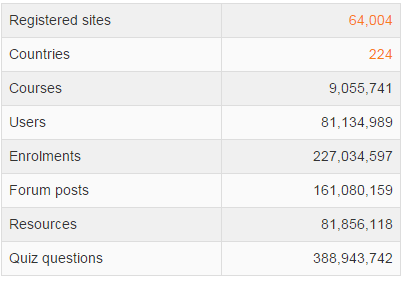
\includegraphics[width=80mm]{images/statistiky-moodle.png}
		   \end{center}
		  \caption{Počet kurzů a uživatelů ze stránek registrovaných na Moodle.org.   \cite{moodle-stats}}
		  \label{fig:moodlestats}
		\end{figure}

V~listopadu roku 2010 vychází verze 2.0 a mění se systém vydávání nových verzí na šestiměsíční cykly. S~novou verzí se Moodle zaměřuje také na mobilní technologie. V~roce 2013 vychází plnohodnotná mobilní aplikace a také šablona vzhledu uzpůsobená zobrazení na mobilních zařízeních.

		

	\section{Vlastnosti Moodlu}
Kapitola shrnuje informace o~licenční politice, komunitním rozvoji a požadavcích pro instalaci a běh aplikace. Zhodnotíme si systém s~jeho výhodami i nevýhodami.
		\subsection{Licence}
Moodle není nijak závislý na licencích za počet uživatelů, přístupů či kurzů. Jedná se o~nezávislý software s~otevřeným zdrojovým kódem (tzv. open source) pod licencí GNU = General Public License (zkráceně GPL), která umožňuje použití pro osobní i komerční užití. Také znamená možnost jakýchkoliv úprav a vlastních doplňků a jejich další šíření, pokud souhlasíte s~tím, že: \emph{„budete tento zdroj poskytovat ostatním; nebudete měnit ani odstraňovat původní údaje o~licencích a autorských právech, a uplatníte stejné licenční podmínky i u~jakýchkoliv odvozených produkt"} \cite{moodle-what-is}. 
		\subsection{Prerekvizity}
Moodle pro svůj provoz nevyžaduje specifický operační systém (je implementován v~PHP) nebo databázi. Není tedy nutné platit za licence dalšího softwaru. Specifikace poslední verze\footnote{V době psaní této práce byla verze Moodle 2.9.3+.}  má následující minimální softwarovou konfiguraci pro provoz \cite{softprereq}:
\begin{itemize}
\item PHP 5.4.4
\item MariaDB 5.5.31 (a vyšší) nebo MySQL 5.5.31 (a vyšší) nebo Postgres 9.1 (a vyšší) nebo MSSQL 2008 (a vyšší) nebo Oracle 10.2 (a vyšší)
\item ostatní softwarové komponenty jsou odvozeny od operačního systému (například jako webový server může být Apache, IIS, Nginx a další) 
\end{itemize}

Mezi minimální hardwarové požadavky patří \cite{hardprereq}:

\begin{itemize}
\item dostatečně velké úložiště na materiály a zdrojové kódy Moodle; 5GB je označeno jako absolutní minimum 
\item odlišné umístění pro zálohování se stejnou nebo větší kapacitou než úložiště výše
\item minimálně 1GHz procesor, doporučuje se 2GHz dual core; skutečné nároky jsou určeny počtem uživatelů a zdrojů
\item systémová pamět minimálně 1GB; skutečné nároky jsou určeny počtem uživatelů a konfigurací stránek
\end{itemize}


		\subsection{Rozvoj}
Rozvoj Moodlu se opírá o~komunitu, kterou tvoří nejen programátoři pracující na Moodle, ale také široká uživatelská základna. Komunita zastává také funkci uživatelského testování se zpětnou vazbou tvůrcům a bugreporting\footnote{hlášení chyb}. Zastává také funkci podpory, kdy si uživatelé navzájem pomáhají a radí, jak řešit problémy. Vedle komunity se během řady let vývoje Moodlu vytvořila skupina komerčních partnerů, kteří nabízejí služby spojené s~Moodlem. Typicky se jedná o~služby, jako je instalace Moodlu, jeho nastavení, spravování, upgrade na novější verze, migrace, hosting, přizpůsobení vzhledu a funkcionality, vývoj nových rozšíření a nadstaveb a další.
		\subsection{Výhody a nevýhody}
Výše zmíněná komunita Moodlu se bezesporu řadí mezi stěžejní výhody, stejně jako sít partnerů. Mezi další výhody Moodlu patří \cite{cooch}:
\begin{itemize}
\item vícejazyčné překlady
\item relativní jednoduchost použití (tento bod jsem doplnil označením relativní, platí dle mého názoru při použití základních struktur a nastavení)
\item škálovatelnost
\item vysoká frekvence oprav a nových verzí (velké verze jsou vydávány dvakrát ročně, opravy pak na téměř denní bázi), které jsou dostupné z~GITu
\item robustnost
\item bezpečnost
\item možnost instalace v~cloudu
\item kompatibilita s~mobilními zařízeními
\end{itemize}


Na druhou stranu má Moodle i své nevýhody. Mezi ně bychom mohli zařadit například:
\begin{itemize}
\item Náročnost na hardware -- zvyšující se počet studentů úměrně zvyšuje nároky na hardware (především systémové paměti)
\item Složitá nastavení -- v~Moodlu můžete nastavením změnit prakticky vše od nadpisu na titulní straně až po logiku vyhodnocení známek a vytvoření webových služeb. Ačkoliv se to může jevit jako výhoda, problém je někdy v~nelogickém pojmenování a vysoké závislosti me\-zi nastaveními. Změna jednoduchého nastavení může mít zpočátku neočekávané následky.
\item Komplikovaná změna vzhledu -- Moodle ve své základní instalaci nevypadá jako moderní graficky přitažlivý systém a dostupné šablony jsou často jen variací tohoto vzhledu. Vytvoření vlastního vzhledu Moodle umožňuje, ale i pro grafika se zkušenostmi s~tvorbou šablon pro Moodle to není jednoduché.
\end{itemize}

Na základě výčtu vlastností výše je zřejmé, že Moodle je skvělým nástrojem pro menší a střední organizace, střední i základní školy, či podporu části výuky na vysokých školách. Je dostupný cenově i požadavky na prostředí. Pokud jej ale chcete používat efektně a efektivně pro velké množství konkurenčně přistupujících uživatelů, nevyhnete se nákladům na kvalitní hardware a správce, často z~řad komerčních partnerů a poskytovatelů služeb spojených s~Moodlem. 

	\section{Kurz}
V~této kapitole probereme výukové moduly (činnosti i studijní materiály), bloky a rozvržení stránky kurzu.  
		\subsection{Rozložení}
Typickým rozložením aplikace je dvou či tří sloupcový layout, ojediněle se vyskytuje layout s~jediným sloupcem. Základem každé stránky Moodle je kontejner pro vložení hlavního obsahu pro danou sekci/stránku. Při vstupu do kurzu se v~něm zobrazí přehled a složení kurzu, v~detailu výukového modulu se zobrazí látka daného modulu, v~případě správy kurzu, modulu, Moodlu atd. je obsahem kontejneru samotný formulář s~nastavením dané položky.

Boční sloupce obsahují tzv. bloky s~kontextovými ovládacími prvky a doplňky (bloky si blíže představíme níže). Bloky je možné umístit do levého i pravého sloupce, čímž ovlivníme, zda výsledný vzhled bude se dvěma nebo třemi sloupci. Není-li do sloupce přidělen alespoň jeden blok, sloupec je skryt. 

U~instalace bez zásahu do nastavení je při zapnutém i vypnutém režimu úprav (přepínač vypíná a zapíná ovládací prvky editace) kurz i jeho nastavení poskládáno do dvou sloupců, hlavního obsahu a kontextové nabídky pro správu kurzu a stránek.

		\subsection{Výukové moduly}
Výukovým modulem je prostor v~kurzu vyplněný specifickým typem činností. Moodle definuje dvě kategorie modulů na základě toho, zda je modul interaktivní, či nikoliv. Vyžaduje-li modul aktivní přístup studenta popř. učitele, řadí se mezi tzv. činnosti. V~opačném případě jde pouze o~pasivní prvek nazývající se studijním materiálem.
Základní instalace Moodlu obsahuje následující výukové moduly (přehled modulů vychází z~\cite{drlik} a zdrojových kódů Moodlu): 

\textbf{Činnosti}:
\begin{itemize}
\item \textbf{Anketa} -- umožňuje učiteli položit otázku s~výběrem z~více odpovědí. Výsledky ankety mohou být studentům zpřístupněny poté, co odpoví, po jistém termínu nebo případně nikdy. Výsledky lze zobrazovat jmenovitě i anonymně.
\item \textbf{Balíček SCORM} -- umožňuje do kurzu vložit výukový balíček ve formátu dle specifikací SCORM a AICC. Jedná se o~soubory, které jsou zabaleny podle standardu pro výukové objekty. Obsah balíčku se zobrazuje postupně a student v~něm může listovat pomocí navigačních prvků. 
\item \textbf{Databáze} -- umožňuje vytvářet, prohlížet a prohledávat kolekci záznamů bez ohledu na jaké jsou téma. Záznamy databáze mohou obsahovat text, obrázky, odkazy, videa a další informace. Vzhled kolekce a jednotlivých zázna\-mů i lze ovlivnit úpravou šablony.
\item \textbf{Dotazník} -- slouží pro získání zpětné vazby od účastníků kurzu. Pro vytvoření dotazníku lze využít různých typů položek včetně výběru z~daných hodnot nebo volné odpovědi. Vyplněné dotazníky mohou být anonymní. Výsledky mohou být k~dispozici i studentům, nebo pouze vyučujícím.
\item \textbf{Externí nástroj} -- umožňuje studentům pracovat s~prostředky a činnostmi na jiných webových stránkách. Nástroj na straně poskytovatele externích služeb musí podporovat specifikaci LTI. Tvůrci kurzu mohou využívat pouze nástroje, které správce stránek přidá do seznamu externích nástrojů.
\item \textbf{Fórum} -- nabízí další komunikační kanál účastníkům kurzu. K~dispozici je několik typů fór: běžné fórum, kde může každý začínat nové diskuse a zapojit se do stávajících; fórum, v~možností vytvořit pouze jednu diskusi; nebo fórum, kde student nejprve odpovídá na sérii otázek sám za sebe předtím, než se mu zobrazí příspevky ostatních diskutujících. Příspěvky mohou být hodnocené a může z~nich vycházet i hodnocení modulu v~rámci kurzu.
\item \textbf{Chat} -- umožňuje účastníkům kurzu diskutovat na webu v~reálném čase. Záznamy z~chatu jsou uloženy a mohou být zpřístupněny všem účastníkům kurzu nebo jen vybraným uživatelům na základě nastaveného oprávnění. Chat je obzvláště užitečný v~případech, kdy se účastníci kurzu nemohou setkávat tváří v~tvář.
\item \textbf{Průzkum} -- poskytuje klasické dotazníky, které se obvykle používají při on-line průzkumech. Učitel je může použít pro sběr údajů od svých studentů ke zlepšení výuky a získání zpětné vazby jak k~obsahu kurzu, tak k~jeho vedení.

\item \textbf{Přednáška} -- umožňuje vytvářet materiál s~posloupnosti stránek a aktivit. Vzniká tak výukový prvek, kterým student může projít celou řadou cest. Jednotlivé stránky lze doplnit interaktivní prvky(např. výběr z~možností, párování a krátké odpovědi), kde v~závislosti na odpovědi a nastavení přednášky mohou studenti postoupit dál.

\item \textbf{Slovník} -- umožňuje vytvářet a udržovat seznam termínů a jejich definic. K~položkám slovníku je možno přikládat soubory. Položky lze  řadit a prohledávat podle různých kriterií (abecedně, kategorie, autor, atd.). Do slovníku mohou přispívat také studenti kurzu a lze nastavit, aby jimi přidané položky vyžadovaly schválení před zobrazením ostatním studentům.

\item \textbf{Test} -- umožňuje vkládat testy skládající se z~výběrových úloh, dichotomických úloh, srovnávacích úloh, úloh s~krátkou tvořenou odpovědí a dalších. Každý pokus o~absolvování testu je automaticky ohodnocen. Učitel může nastavit počet povolených pokusů, zpětnou vazbu, zobrazení správných odpovědí, úlohy zamíchat nebo náhod\-ně vybírat z~banky úloh. Může být nastaven časový limit pro testování. Každý pokus hodnotí automaticky kromě dlouhé tvořené odpovědi.

\item \textbf{Úkol} -- umožňuje učiteli zadat úkoly, hodnotit odevzdané řešení a komentovat je. Studenti mohou odevzdat libovolný soubor, jako dokumenty textových aplikací, tabulky, obrázky nebo audio a video. Alternativně nebo současně může úkol požadovat, aby studenti napsali text přímo do textového pole. Úkol může být použit také pro připomenutí jiných povinností studentů, které neprobíhají přímo v~Moodle - např. odevzdání výkresu. Úkoly mohou být klasifikovány jednoduchým přímým hodnocením, případně pokročilou metodou. Výsledná známka je zapsána do klasifikace.

\item \textbf{Wiki} -- umožňuje pracovat s~články v~rámci encyklopedie podobně jako na portálu Wikipedia\footnote{\url{https://wikipedia.org/}}. Modul Wiki může pracovat ve dvou režimech: kolaborativníim (každý má možnost úpravy), nebo v~individuálním (každý má svou wiki).

\item \textbf{Workshop} -- umožňuje sběr a vzájemné hodnocení prací studentů. Studenti mohou odevzdat libovolný obsah (dokumenty, obrázky, video nebo text psaný přímo v~editoru). Studenti mají možnost hodnotit jednu nebo více přidělených prací. Odevzdaná řešení i jejich hodnocení mohou být anonymní. Patří k~nejvíce komplikovaným modulům z~hlediska nastavení i následného používání.
\end{itemize}

\textbf{Studijní materiály}:
\begin{itemize}
\item \textbf{Kniha} -- umožňuje vytvořit vícestránkový studijní materiál s~obsahem děleným na kapitoly a podkapitoly.  Jsou vhodné zejména při práci s~delším textem nebo skriptem, který učitel rozděli na kapitoly tak, aby text zůstal přehledný i v~elektronické podobě.
\item \textbf{Popisek} -- umožňuje do osnovy kurzu vložit stručný text, obrázek, video nebo odkaz další činnosti. Slouží především k~vylepšení vzhledu kurzu.
\item \textbf{Složka} -- umožňuje učiteli vytvořit strukturu ke sdílení více dokumentů na jednom místě tak, aby student nemusel hledat v~kurzu umístění jednotlivých dokumentů. Více souborů najednou lze nahrát pomocí ZIP archívu.
\item \textbf{Soubor} -- umožňuje učiteli poskytnout soubor jako studijní materiál. Pokud je to možné, bude soubor zobrazen jako součást kurzu, jinak budou studenti vyzváni k~jeho stažení.
\item \textbf{Stránka} -- umožňuje učiteli vložit webovou stránku pomocí editoru. Stránka může jakýkoliv zdrojová kód  od textu, obrázků či odkazů po zvuk, Youtube video nebo Google prohlížeč map.
\item \textbf{URL} -- umožňuje učiteli použít webový odkaz v~těle kurzu, který směřuje i mimo web\-ové stránky Moodlu.
\end{itemize}
Výčet modulů však není konečný a lze je rozšířit o~další moduly dostupné z~Moodle databáze\footnote{Databáze modulů a pluginů je dostupná z~\url{https://moodle.org/plugin}, případně u~poskytovatelů třetích stran.} nebo vývojem vlastních rozšíření.

		\subsection{Bloky}
Vedle výukových modulů, které jsou jednoznačně určené k~tvorbě obsahu kurzu, stojí tzv. bloky usnadňující uživateli práci s~kurzem a systémem jako takovým. Typickým příkladem bloku jsou kontextová menu Správa kurzu a Správa stránek, které je viditelné při spuštěném Režimu úprav. Mezi bloky nabízené v~„holé” instalaci patří kalendář obsahující termíny plnění úkolů, testů, začátek či konec kurzu a další data, která se týkají právě přihlášeného uživatele. Blokem ale může být téměř cokoliv, HTML kód, zobrazení posledního přidaného úkolu nebo kurzu, zobrazení anket, odkazů, kontextové menu a další.
	\section{Uživatelské role a kontext}
Moodle definuje uživatelskou roli ve spojení s~kontextem. Kontext ohraničuje části systému a umožňuje těmto částem přidělovat různé vazby uživatele s~rolí. Příkladem může být kategorie kurzů, která má svůj vlastní kontext. Kategorie obsahuje kurzy, které mají také svůj kontext. V~kurzech se vytváří aktivity a materiály, mimo stojí tzv. bloky. I~tyto části kurzu mají svůj vlastní kontext. K~těmto kontextům nyní můžeme přiřadit uživatele ve vazbě s~rolí. Uživatel tedy může být v~kontextu kurzu A~definován jako učitel a v~kontextu kurzu B jako student. V~rámci kurzu B může náš uživatel mít v~kontextu modulu diskuze roli moderátora. 

Globální roli má uživatel zapsanou bez ohledu na kontext a je platná bez ohledu na místo, kde se uživatel právě nachází. Lokální role se naopak zapisuje v~rámci kontextu a tím se vytváří systém práv ke každé stránce v~daném kontextu. Práva mohou být přebírána z~jiných kontextů, jelikož Moodle vytváří nad kontexty hierarchii (obrázek \ref{fig:moodlecontext}). Přebírání práv je však možné směrem dolů. Směrem do strany (sdílení mezi kontexty stejné úrovně) a nahoru (do nadřazeného kontextu) nelze. Moodle k~uživatelským rolím uchovává informaci o~případném archetypu. Archetypem se myslí rodičovská skupina, ze které role vychází a dědí z~ní základní množinu vlastností. 
 

		\begin{figure}
		  \begin{center}
		    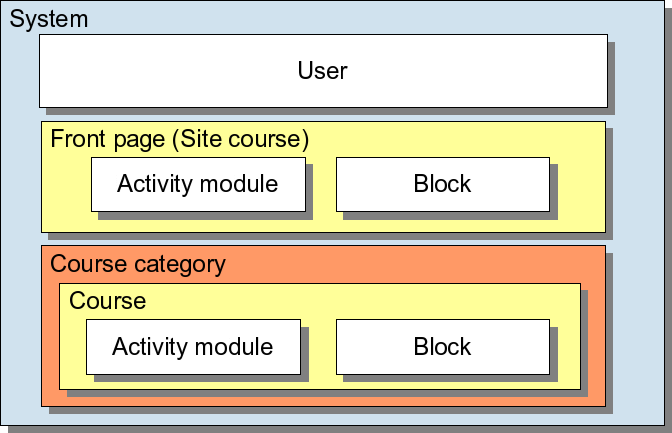
\includegraphics[width=120mm]{images/moodle-context.png}
		   \end{center}
		  \caption{Grafické zobrazení hierarchie kontextů.   \cite{moodle-context}}
		  \label{fig:moodlecontext}
		\end{figure}
Základní instalace Moodle obsahuje tyto role:
\begin{enumerate}
\item \textbf{Administrátor (administrator)} \\*Uživatel v~této roli má neomezený přístup (nekontrolují se u~něj přístupová práva) ke všem možnostem a nastavením v~Moodlu. Jako hlavní správce systému: \begin{itemize}
	\item vytváří, maže a spravuje ostatní uživatele (Správa uživatelů)
	\item nastavuje systémové vlastnosti, řídí zálohování a upgrade systému (Správa systému)
	\item vytváří, importuje a exportuje kategorie kurzů a kurzy samotné, nastavuje přístupy a uživatelské skupiny (Správa kurzů)
\end{itemize}
\item \textbf{Manažer (manager)} \\*Manažeři mají právo přistoupit do jakéhokoliv kurzu, upravit jeho složení a nastavení, popřípadě odstranit nebo přidělit další uživatele kurzu v~kontextu Kategorie kurzů a stává se „administrátorem kurzů”. Manažer v~kurzu nebývá zapsaným uživatelem.
 	
\item \textbf{Tvůrce kurzu (coursecreator)} \\*Role slouží k~přidělení práv na vytváření kurzů v~kontextu Kategorie kurzů. Uživatel s~tímto oprávněním kurzy vytváří, nastavuje obecné vlastnosti (název, kategorii, začátek kurzu, viditelnost atd.), vzhled, uspořádání kurzu, přístupy, zapsání uživatelů a další. Přidává do jednotlivých sekcí (na základě uspořádání) moduly i s~jejich nastavením a pravidly pro hodnocení a bloky zobrazené v~kurzu. Uživatel s~touto rolí může vystupovat jako učitel a definovat další učitele.
	
\item \textbf{Učitel (editingteacher)} \\*
	Učitelé mohou v~rámci kurzu prakticky vše. Vytvářet, měnit a odebírat moduly a bloky kurzu, měnit pravidla pro hodnocení modulů, provádět změny podmínek pro zápis do kurzu a jiné. Role učitel je přiřazena v~kontextu Kurzu. 

\item \textbf{Učitel bez práva upravovat (teacher)} \\*
	Učitel bez práva upravovat je stejně jako učitel přiřazen v~kontextu Kurzu. Rozdíl oproti učiteli je právě v~odebrání možnosti upravovat nastavení kurzu a aktivit. Učiteli bez práva upravovat zůstávají práva učit v~kurzu, moderovat diskuze, komentovat a známkovat výkony studentů.

\item \textbf{Student (Student)} \\*
	Student je role definovaná na úrovni kontextu Kurzu a opravňuje uživatele se zapisovat do kurzů a plnit aktivity. Mají žádná nebo minimální práva k~editaci a v~rámci kontextů jednotlivých aktivit mohou mít přidělena další práva (editaci databáze slov, přidávání odkazů, moderování diskuzí apod.).

\item \textbf{Host (Host)} \\*Host je neregistrovaný uživatel s~právem nahlížet na hlavní stránku Moodlu, popřípadě s~právem nahlížet do kurzů, které mají nastavená práva pro hostující uživatele.

\item \textbf{Registrovaný uživatel (Registered user)} \\*Roli automaticky získávají všichni uživatelé, kteří mají založený účet.

\end{enumerate}


	\section{Vytvoření kurzu a jeho nastavení}
Vytvoření nového kurzu v~prostředí LMS Moodle je jednoduchý proces, kte\-rý spočívá ve vyplnění jednoho formuláře. I~přesto ukrývá nástrahy v~podobě skrytých nebo nedostatečně vysvětlených nastavení a může způsobit neočekávané potíže i zkušenému tvůrci kurzů (ačkoliv to platí především pro nastavení jednotlivých modulů). Moodle je nechvalně známý svou složitostí a závislostí nastavení, obzvláště v~oblasti hodnocení kurzu a modulů. Z~tohoto důvodu si proces vytvoření nového kurzu projdeme i s~vysvětlením základních nastavení.
		\begin{figure}
		  \begin{center}
		    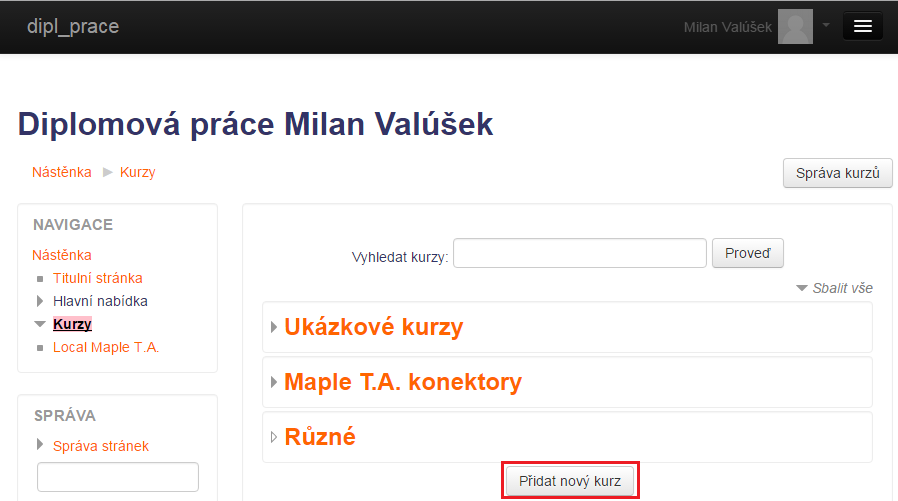
\includegraphics[width=120mm]{images/kurzy-pridani.png}
		   \end{center}
		  \caption{Náhled obrazovky s~kategoriemi kurzy (uživatel s~právy vytvořit kurz).  }
		  \label{fig:moodlekurzypridani}
		\end{figure}
\subsection*{Přidání kurzu}
Pro vytvoření nového kurzu musí být přihlášený uživatel zapsán v~roli, kte\-rá umožňuje tvorbu kurzů. Uživateli s~příslušnými právy se na stránce s~přehledem kurzů zobrazuje tlačítko Přidat nový kurz (obrazek \ref{fig:moodlekurzypridani}). Po stisknutí tlačítka se zobrazí veškerá nastavení kurzu po následujících záložkách (obrázek \ref{fig:moodlekurzypridanidetail}):
 

\subsection*{Obecná nastavení}
V~této části musí být nastaveny povinné „iniciály kurzu”, mezi které patří následující atributy:
\begin{itemize}
	\item Celý název -- zobrazuje se v~horní části kurzu a v~seznamech kurzů
	\item Krátký název kurzu -- je označení kurzu tam, kde není potřeba celého názvu. V~tomto atributu může být zkratka nebo kódové označení (např. PB001, MAT1, apod.).
\end{itemize}
Mezi nepovinné nastavení v~této části patří:
\begin{itemize}
	\item Kategorie kurzu -- do které má být nový kurz přidán
	\item Viditelný -- atribut určující viditelnost v~seznamech dostupných kur\-zů. Neviditelný kurz uvidí pouze administrátor a učitelé zapsaní do daného kurzu.
	\item Datum začátku kurzu -- určuje, odkdy mohou studenti začít s~kurzem pracovat
	\item Identifikátor (ID) kurzu -- označení v~případě propojení s~externími systémy
\end{itemize}
\subsection*{Popis}
Popis obsahuje nastavení anotace kurzu (Shrnutí kurzu) a zobrazuje se společně s~názvem kurzu. K~anotací se v~této části dá přidat navíc ještě soubor (například obrázek), který je zobrazen se shrnutím kurzu.

\subsection*{Typ uspořádání kurzu}
Moodle nabízí čtyři typy uspořádání kurzu a na základě výběru se mění další nastavení. Mezi typy kurzů patří:
\begin{itemize}
	\item Týdenní uspořádání -- sekce kurzu jsou rozděleny na týdny počínaje dnem začátku kurzu. Dále uživatel zadává počet sekcí (týdnů), které se připraví, a zda se budou neaktivní týdny zobrazovat rozbalené. Posledním nastavením je stránkování, tedy jestli budou všechna témata na jedné stránce nebo se každé bude zobrazovat na samostatné stránce.
	\item Tematické uspořádání -- je rozdělení do více témat, kde téma není omezeno časově, ale zaměřením na konkrétní látku. Další nastavení jsou stejná jako v~případě týdenního uspořádání.
	\item Formát jednoho modulu -- vytvoří kurz s~jedním jediným modulem. Používá se například při vytváření kurzu z~tzv. SCORMů, ale může to být kterýkoliv dostupný modul. A~právě výběr použitého modulu je jako další nastavení.
	\item Diskuzní uspořádání -- znamená, že na stránce kurzu jsou zobrazeny diskuze. Další nastavení určuje, kolik jich bude zobrazeno.
\end{itemize}
\subsection*{Ostatní nastavení}
Nastavení ostatních záložek je totožné pro všechny kombinace dalších nastavení. Počet a význam nastavení není natolik zásadní, abychom se jim věnovali samostatně po blocích, proto je shrneme společně:
\begin{itemize}
	\item Vnutit jazyk (Vzhled) --pole obsahuje volbu překladu na základě nainstalovaných jazykových mutací. Jako výchozí nastavení je možnost Nevnucovat, která jazyk přizpůsobí podle nastavení profilu uživatele. Při výběru konkrétního jazyka se kurz snaží přizpůsobit zvolené mutaci.
	\item Kolik novinek ukazovat (Vzhled) -- určuje, kolik novinek se bude zobrazovat v~bočním sloupci kurzu. Při výběru 0 sloupec zmizí.
	\item Ukázat známky (Vzhled) -- nastavení zobrazení známkování u~činností, které jsou známkovány.
	\item Ukázat sestavu o~činnosti (Vzhled) -- nastavení zobrazení činnosti studenta v~kurzu. Moodle si při práci s~činnostmi ukládá záznam pro každého uživatele.
	\item Maximální velikost nahrávaných souborů (Soubory a nahrávání) -- nastavení limitu velikosti nahrávaného souboru do kurzu. Například při odevzdávání úkolů nebo uploadu materiálů.
	\item Povolit přístup pro hosty (Přístup pro hosty) -- nastavení, zda mohou do kurzu vstoupit neregistrovaní uživatelé. 
	\item Heslo (Přístup pro hosty) -- heslo je neaktivním nastavením až do chvíle, kdy povolíte přístup pro hosty. Jeho nastavení slouží hostům k~primitivní autentizaci.
	\item Přejmenování rolí -- ve skupině je možné pro uživatelské role použít jiná označení. Nastavení využijete, například pokud nechcete mást uživatele novým označením některé role. Používá-li organizace pro učitele v~kurzu označení „tutor”, využije právě této možnosti. 
\end{itemize}
		\begin{figure}
		  \begin{center}
		    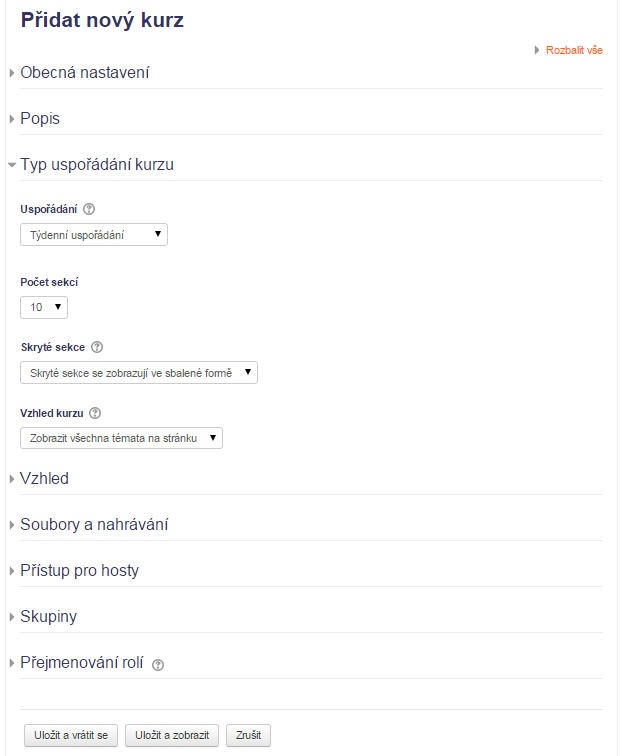
\includegraphics[width=120mm]{images/kurzy-pridani-detail.png}
		   \end{center}
		  \caption{Náhled na formulář pro přidání kurzu.}
		  \label{fig:moodlekurzypridanidetail}
		\end{figure}

Po nastavení potřebných atributů můžete kurz uložit a dokončit tím jeho tvorbu. K~nastavení se můžete kdykoliv vrátit a přizpůsobit jej dalším potřebám. Po vytvoření kurzu lze začít s~přípravou jeho obsahu zapnutím režimu úprav a vytvořením požadovaných výukových modulů.


\chapter{Maple T.A.}
V~této kapitole si představíme nástroj Maple T.A. a popíšeme jeho základní vlastnosti.
	\section{Co je to Maple T.A.?}
Maple T.A. patří do rodiny nástrojů Maple společnosti Maplesoft, která je jedním z~předních dodavatelů softwaru pro strojírenství, matematické a vědecké účely. Zkratka T.A. pochází z~anglického Testing and Assessment (testování a posuzování) a doplňuje řadu produktů společnosti Maple o~e-learn\-ingový systém.

		\begin{figure}
		  \begin{center}
		    
\includegraphics[width=80mm]{images/MapleTA_logo.jpg}
		   \end{center}
		  \caption{Oficiální logo Maple T.A.  \cite{maple-logo}}
		  \label{fig:maplelogo}
		\end{figure}

Maple T.A. je webová aplikace pro vytváření otázek a cvičení s~automatickým hodnocením odpovědí. Odpověď může být předána jednoduchým výběrem ze dvou a více odpovědí nebo komplexní formou v~podobě vytvářené matematické formulace, kterou Maple pomocí pokročilého vyhodnocení zpracuje a rozhodne o~správnosti odpovědi. Není nutná jediná přesná forma odpovědi, korektní ekvivalent odpovědi bude také vyhodnocen jako správný. Maple navíc může otázky generovat na základě předem definovaných šablon, čímž se snižuje pravděpodobnost, že by dva studenti jedné třídy dostali v~rámci jednoho úkolu stejný příklad.\cite{heck2004}

Zaměření Maple T.A. je cíleno na kurzy zahrnující matematiku. Jeho jedinečné vlastnosti umožňují učiteli zadávat úkoly a příklady v~podobě, která od studentů vyžaduje pochopení matematických konceptů, a dělají z~něj ideální nástroj pro vědecké, technické, strojírenské a matematické (STEM - science, technology, engineering and mathematics) kurzy. I~přesto, že Maple T.A. je samostatně fungující platforma a nástroj pro správu matematicky orientovaných kurzů, podporuje integraci svých funkcí s~ostatními nástroji. \cite{mapleta} 


Ve srovnání s~Moodlem je Maple T.A. zaměřený především na procvičování, zkoušení a testování než na samotnou výuku. Aplikace dovoluje vkládat materiály a vytvářet tok informací ke studentovi, tak aby danou problematiku pochopil, ale její koncept k~tomuto nebyl vytvořen. Naopak se očekává, že uživatelé aplikace mají základy dané problematiky a v~aplikaci probíhá procvičování a evaluace probrané látky.


	\section{Licencování}

Maple T.A. není, na rozdíl od Moodlu, open source ani freeware. Jedná se o~licencovaný software s~více licenčními možnostmi. Prakticky nabízí tři scénáře licencování softwaru  \cite{mapletalicence}:
\begin{enumerate}
	\item Hostování Maplesoftem na čas -- aplikace běží na serverech Maplesoftu, který se stará o~nastavení aplikace, integraci s~ostatními systémy, instalaci záplat a nových verzí, jakmile je to možné (po dohodě se zákazníkem). Licence je omezena časově, ale i počtem studentů, kteří za danou dobu přistoupí do systému. Počet licencí pro přístup a obnovení licence je možné na základě potřeb zákazníka a může být účtováno po třídách, odděleních nebo za celou instituci.
	
	\item Hostování Maplesoftem dle velikosti -- aplikace běží na serverech Maplesoftu, který se stará o~nastavení aplikace, integraci s~ostatními systémy, instalaci patchů a upgradů, jakmile je to možné (po dohodě se zákazníkem). Instituce platí administrativní poplatek za vytvoření třídy a studenti si kupují licenci pro přístup do aplikace.
	
	\item Vlastní instalace -- instalace běží na serveru instituce a veškeré administrativní zásahy, nastavení, instalace nových verzí a záplatování je v~kompetencích instituce. Hlavní záplaty a verze obdrží zákazník pouze v~případě, že má zaplacené předplatné programu Maplesoft Elite Maintenance Program\footnote{Program pro podporu aktualizace softwaru poskytovaného společností Maplesoft, založený na bázi roč\-ního předplatné.} (dále jen EMP) nebo si je může přikoupit zvlášť. Na programu EMP je založeno i nasazení nového obsahu. Možnost rozvoje obsahu není omezena, ale nasazení obsahu do produkce (tak, aby jej studenti mohli používat) je podmíněno aktivním předplatným EMP. EMP zákazník získává automaticky na první období při zaplacení licence. Licence je v~tomto případě poskytována na počet studentů, kteří mohou systém používat, a může být v~případě zájmu rozšířena. Účtování může být opět rozvrženo na třídu, oddělení (část instituce) nebo celou instituci.
\end{enumerate}


	\section{Předpoklady pro instalaci}
Maple T.A. je implementován v~jazyce Java, což umožňuje jeho instalaci na servery rozdílných platforem, kde lze nainstalovat Javu a aplikační server Tomcat. Minimálními softwarovými požadavky pro běh aplikace na vlastním serveru jsou \cite{mapletarequirements}:
\begin{itemize}
	\item Oracle Java 6 nebo 7 (bez rozdílu použití Java Development Kit nebo Java runtime environment\footnote{Java runtime environment (JRE) je knihovna pro spouštění aplikací v~Javě a Java Development Kit (JDK™) je knihovna pro vývoj aplikací v~Javě obsahující JRE})
	\item aplikační server Tomcat 6.0 nebo 7.0.
	\item databázový server PostrgreSQL 9.3
\end{itemize}

Kromě softwarových požadavků je potřeba splnit i minimální hardwarové požadavky:
\begin{itemize}
	\item minimálně dvoujádrový procesor (doporučený je osmijádrový)
	\item minimálně 2 GB RAM (doporučeno mít 32 GB)
	\item minimálně 20 GB volného místa na pevné paměti (doporučeno 40 GB)
	\item jednotlivé platformy mohou požadovat drobné dodatečné konfigurace
\end{itemize}
	\section{Základy aplikace}
Koncept výuky v~Maple T.A. se zakládá na třídách. Třída je, stejně jako ve škole, skupina žáků, která dostává stejné učební materiály, úkoly a testy, na jejichž základě je žák hodnocen. Každá třída má úložiště dokumentů, ve kterém mohou učitelé sdílet materiály se svými studenty. V~následující části si vysvětlíme základní pojmy používané v~rámci procesu výuky a testování.
		\subsection{Otázka (Question)}
Lepším označením než otázka by mohla být například testovací jednotka, jelikož představuje komplexní objekt, který v~sobě skrývá kromě samotné otázky také klíč k~vyhodnocení, popis, zpětnou vazbu, ohodnocení a další. Otázky tvoří základní prvek aplikace a provádí auto-evaluaci odpovědí (výsledky úloh nejsou vyhodnocovány učitelem) s~výjimkou tvořených úloh (eseje, tvořené odpovědi apod.) \cite{crompton}. Příprava nových otázek vyžaduje znalosti a zkušenosti nejen v~oblasti, pro kterou jsou otázky tvořeny (matematika, fyzika, strojírenství apod.), ale také se samotným nástrojem pro vytváření a editování. Zadávání otázek lze prakticky provést třemi možnými způsoby \cite{heck2004}:

\begin{enumerate}
	\item on-line pomocí editoru otázek (Question Bank Editor)
	\item za využití syntaxe Maple skriptovacího jazyka (dostupné on-line i off-line)
	\item použitím LaTeXu a specifických maker se vytvoří skript, které se do systému nahrají z~Internetu
\end{enumerate}
První z~metod je nejoblíbenější a nejjednodušší na použití. U~zbylých dvou metod je nutné znát syntaxi skriptovacího jazyka používaného Maplem, popřípadě maker k~vytvoření otázky. Přestože způsob zadávání otázek pomocí vlastních skriptů je náročný na tvůrce, je vhodný pro zadávání komplexních otázek založených na specifických algoritmech vyhodnocení. Tímto způsobem totiž vznikají otázky, u~kterých autor může využít knihoven a modulů přímo z~jádra (engine) Maplu \cite{char}. Vytváření otázek pomocí skriptovacího jazyka Maplu je velice komplexní a obsáhlá problematika a pro potřeby práce nám postačí základní vestavěné typy (typům úloh se budeme věnovat v~kapitole \ref{sec:typyuloh}). 

		\subsection{Úkol (Assignment)}
Úkol jako takový je obálkou, kterou vyplníme základní informace a název, vložíme do ní otázky a vybereme typ úkolu, průchod úkolem je po jeho vytvoření automatizovaný. Typ úkolu definuje prostředí a proces, jakým bude prováděno testování. Maple T.A. nabízí následující typy:

\begin{itemize}
	\item Studium/samostudium
	\item Procvičování
	\item Domácí úkol / test
	\item Zkouška s~dozorem 
	\item Mastery dialog
\end{itemize}
Úkolům se budeme blíže věnovat v~kapitole \ref{sec:vytvoreniukol}.

	\subsection{Kniha hodnocení (Gradebook)}
Kniha hodnocení je nástroj, který sjednocuje výsledky studentů k~prohlížení a analýze. Po dokončení průchodu úkolem jsou zaznamenané hodnoty zobrazeny právě v~knize hodnocení. Nástroj z~informací vytváří statistiky studentů, úkolů a otázek, ze kterých generuje reporty o~jednotlivých studentech, třídách nebo pro výběr více tříd. Vytvořením politiky známkování může instruktor vytvořit různé váhy známky z~úkolů a na základě této politiky poté exportovat známky do souboru nebo je publikovat studentům k~prohlížení. Kniha umožňuje dodatečné úpravy známek a přidání hodnocení, která nejsou založena na průchodu úkolem (prezentace, ústní zkoušení, příprava materiálů atd.).
	\section{Typy úloh} \label{sec:typyuloh}

V~této kapitole si představíme základní typy vestavěných otázek, které se v~Maple T.A. mohou vyskytnout (celá kapitola vychází z~\cite{maple-question} a \cite{char}):

	\subsection{Volná matematická odpověď}
Maple T.A. umožňuje ptát se na otázky s~volnou odpovědí, u~nichž student odpovídá stejně, jako by se jednalo o~papírovou práci. Matematickou notaci lze využít jak při vytváření otázky, tak při psaní odpovědi, jelikož editor matematických formulí zjednodušuje zadávání matematických výrazů. Otázky jsou navíc hodnoceny nejen na základě definovaného řetězce, matematický preprocesor umožňuje označení korektní odpovědi i v~případě matematického ekvivalentu. Například pokud je správnou odpovědí jedna pětina, a student odpoví, že správně jsou dvě desetiny, Maple T.A. ji vyhodnotí také správně. Otevřené otázky mohou mít i nekonečnou množinu správných odpovědí (například: \emph{„Uveďte funkci, která má maximum v~x = 0”}). Otázky mohou být prakticky z~jakékoliv oblasti matematiky a Maple T.A. je bude schopen vyhodnotit a oznámkovat automaticky.


	\subsection{Adaptivní otázky}
Maple T.A. poskytuje adaptivní otázky i celé úkoly. Adaptivní otázka znamená, že pokud má student problém odpovědět správně, otázka mu napomáhá dle nastavení instruktora, například:
\begin{itemize}
	\item v~otázce se uvedou podrobnosti k~tomu, jak ji řešit
	\item zadá studentovi jednodušší verzi otázky
	\item provede ho po menších krocích řešení
	\item nechá ho otázku řešit znovu se sníženým koeficientem
	\item ostatní
\end{itemize}

Ostatní způsoby jsou již na uvážení instruktora, který může rozhodnout o~dalším chování. Příkladem může být nastavení počtu opakování pro různé části, kdy se nabídne jiné řešení, či údaj, kolikrát může student zadat nesprávnou odpověď, a podobně.

	\subsection{Kreslení grafů}
Kreslení grafů je velice zajímavé řešení otázky, které Maple T.A. opět dokáže vyhodnotit samostatně. Grafem, který má student nakreslit, může být prakticky cokoliv. Od zadání bodu po náčrt asymptot, parabol a intervalů. Student zadává odpovědi kliknutím na klíčové body v~grafu, zadáním dvou bodů pro zakreslení přímky nebo bodu a vrcholu pro parabolu. V~zadání otázky mohou být některé linky v~grafu zakresleny a student má určit některé další informace (například kudy bude procházet tečna k~dané křivce). 
		\begin{figure}[hbt]
		  \begin{center}
		    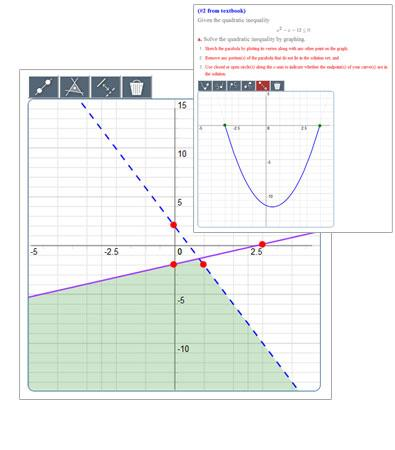
\includegraphics[width=90mm]{images/MapleTA_graph.png}
		   \end{center}
		  \caption{Otázka s~kreslením grafu.  \cite{maple-question}}
		  \label{fig:maplegraph}
		\end{figure}

	\subsection{Volný náčrt}
Dalším typem otázek je volné zakreslení křivek do obrázku nebo načrtnutí diagramu. Po studentovi se v~tomto typu obvykle požaduje vytvoření čar nebo křivek na základě připraveného zadání. Typickým příkladem může být zadání, v~němž má student uvést, kterým směrem působí síly odstředivé a dostředivé, do obrázku pneumatiky auta. Student kreslí šipky přímo do obrázku a vyhodnocení může být s~tolerancí.
  		\begin{figure}[hbt]
		  \begin{center}
		    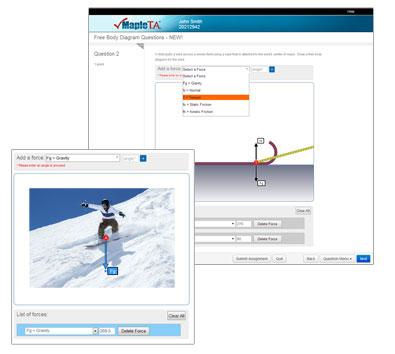
\includegraphics[width=90mm]{images/MapleTA_paint.png}
		   \end{center}
		  \caption{Otázka s~volným náčrtem.  \cite{maple-question}}
		  \label{fig:maplepaint}
		\end{figure}

	\subsection{Obrázek k~doplnění}
Učitel nahraje do systému jakýkoliv obrázek a v~editoru vytvoří místa, na která student může kliknout. Zadáním může být například výběr správné planety ze sluneční soustavy, umístění ledvin v~lidském těle nebo ohnisko elipsy.
 
	\subsection{Matematické aplikace}
Matematickou aplikací je úloha, ve které student pomocí interaktivních prv\-ků zadává řešení a na základě vstupu se mění další hodnoty, grafy nebo zobrazení. K~zadání výsledku v~úloze mohou být připravena pole pro doplňování hodnot nebo osy pro přetažení posuvníku. Maple T.A. úkoly tohoto typu hodnotí automaticky a proměnné v~zadání mohou být generovány tak, aby vznikla množina unikátních zadání stejného typu.
		\begin{figure}[hbt]
		  \begin{center}
		    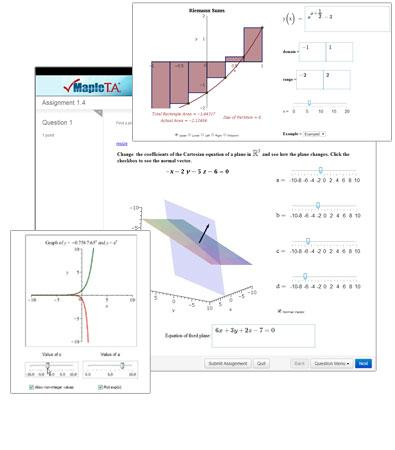
\includegraphics[width=90mm]{images/MapleTA_math.png}
		   \end{center}
		  \caption{Otázka s~kreslením grafu.  \cite{maple-question}}
		  \label{fig:maplemath}
		\end{figure}

	\subsection{Číselná odpověď s~definovatelnou odchylkou}
Odpovědí na otázky jsou v~tomto případě číselné hodnoty, u~nichž může být definována odchylka nebo přesnost, podle které budou hodnoceny jako správné (například výsledek musí být přesný na dvě desetinná místa). Číselné odpovědi systém uznává v~decimálním i vědeckém zápisu čísel a podporuje zadání a převod jednotek během vyhodnocení.

	\subsection{Výběr více správných odpovědí}
Jedná se o~klasický výběr testových otázek, ze kterých student dle nastavení vybírá jednu či více správných odpovědí (zahrnuje otázky s~jednou správnou odpovědí a více správnými odpověďmi ano/ne). Hodnoty proměnných v~otázce i ve výsledcích mohou být automaticky generovány a jsou i automaticky vyhodnoceny.

	\subsection{Doplňování}
Student dostane úlohu s~chybějícím slovem či frází a jeho úkolem je text vhodně dopsat nebo vybrat ze seznamu. Pro vyhodnocení může být zadána jen jedna konkrétní forma, nebo může jít o~celý slovník korektních slov či frází.
 
	\subsection{Esej}
Posledním typem úlohy je esej. Jedná se o~dlouhé tvořené odpovědi, jakým může být například matematický důkaz nebo popis algoritmu. Esej je také jediný typ úlohy, který vyžaduje hodnocení instruktora. Jakmile student dokončí úlohu, jeho odpověď se automaticky odešle instruktorovi k~hodnocení. Pro rychlou orientaci a přehled je tento typ otázek v~knize známek zvýrazněn.



	\section{Uživatelské role}
V~nabídce základní instalace je celkem pět definovaných rolí; ty mohou být volně kombinovány a uplatňovány v~rámci kontextu na třech úrovních (systém, třída, student). Uživatel s~více rolemi může mít v~rámci jedné třídy práva studenta, ve druhé být instruktorem a ve třetí figurovat jako zkoušející. Záleží na kontextu, v~němž je role uživateli přidělena. Od verze 10 nabízí Maple T.A. také možnost vytváření vlastních rolí, u~kterých se omezí/rozšíří práva oproti výchozím rolím. Mezi základní role patří:
\begin{enumerate}
\item \textbf{Student (student)} -- výchozí studentská role. Uživatel na úrovni třídy získává práva měnit svůj profil, přístupy k~materiálům a zveřejněným úkolům na stránce třídy a možnost prohlížet si známky a reporty z~knihy hodnocení.
\item \textbf{Host (guest)} -- role bez jakýchkoliv práv. Slouží jako role pro prohlížení míst, která mají povolený přístup pro hosta.
\item \textbf{Instruktor (instructor)} -- ze systémových práv má právo vytvářet no\-vé kořenové třídy. Na kontextové úrovni třídy vytváří nové otázky a spravuje úkoly, využívá možností knihy hodnocení a zapisuje uživatele (již existující) do rolí student nebo zkoušející. Má právo vytvářet potomky tříd .
\item \textbf{Dozor/zkoušející (proctor)} -- uživatel, který autorizuje studenty ke složení zkoušky nebo úkolů s~omezením přístupu.
\item \textbf{Správce systému (administrator)} -- nejvyšší role přiřazená na úrovni systému. Opravňuje uživatele k~nastavení všech systémových vlastností, k~plné správě (vytváření, úpravě a mazání) uživatelských účtů a kořenových tříd. Při vytváření tříd vybírá instruktora.
\end{enumerate}

	\section{Vytvoření úkolu} \label{sec:vytvoreniukol}

Co je to úkol, jsme si vysvětlili výše, nyní se podíváme blíže na jeho možnosti při vytváření. Maple T.A. vedle klasického pojetí úkolu nabízí variantu tzv. adaptivních úkolů. Rozdíl mezi klasickou a adaptivní formou se skrývá v~tom, že klasická úloha udržuje náročnost úloh na stejné úrovni pro všechny žáky ve všech průchodech úkolem, zatímco adaptivní úkol svou náročnost mění dle úspěšnosti studenta při odpovědích. Slabším studentům při neúspěšnosti náročnost snižuje, tak aby je nedemotivoval v~plnění úloh a umožnil jim dojít složitějších úkolů. Šikovnější studenty naopak posouvá dál a probouzí kreativitu zvyšováním náročnosti úloh a kombinací s~další látkou. 

Pro vytvoření nového nebo úpravu existujícího úkolu si otevřeme třídu, ve které budeme s~úkolem pracovat. Zvolíme, jakou formu – klasickou, nebo adaptivní – bude úkol mít, a započneme tvorbu. Příprava úkolu je rozdělena do následujících čtyř fází:

\subsection*{Pojmenování}
Ve fázi pojmenování vytvoříme kontejner úlohy. Přiřadíme jí název, krátký název (slouží například v~drobečkových navigacích ) a popis úkolu. Kromě těchto základních atributů lze úkolu vyplnit hlavičku a patičku, která se zobrazuje na každé straně úkolu.

\subsection*{Výběr otázek}
Druhou fází přípravy úkolu je výběr otázek. Výše jsme zmínili úkoly adaptivní a klasické, rozdíl v~jejich přípravě leží právě v~této fázi. U~klasického pojetí se ve fázi výběru otázek přiřadí seznam otázek, které se v~úkolu zobrazí, a nastaví se jim bodové ohodnocení. U~adaptivních úloh se otázky vybírají do několika seznamů, jež se ohodnotí koeficientem náročnosti. Poté se nastaví pravidla pro snížení/zvýšení náročnosti (počet správných/špatných odpovědí), oznámkování (známkovat po stanoveném počtu chybně zodpovězených/správně zodpovězených/zobrazených otázek) apod.

\subsection*{Nastavení průchodu}
Máme připravený kontejner na úlohy a vložili jsme do úkolu úlohy k~plnění. Nyní nám chybí ještě rozhodnout a definovat, jaký má daný úkol účel, očekávaný průběh a výstup. Maple T.A. nabízí následující možnosti: 
\begin{enumerate}
	\item Studium/samostudium -- z~výsledků úkolu se nevytváří záznam a neomezuje se počet průchodů. Nenastavují se další práva ani nastavení průběhu a při plnění úkolu se postupně zobrazují informace k~řešení jednotlivých úloh.
	\item Procvičování -- výsledky nejsou v~záznamu průchodu. Procvičování představuje formu klasického testu nanečisto.
	\item Domácí úkol/test -- u~této formy jsou výsledky uloženy. Tvůrce úkolu má několik možností ovlivnit formu úkolu, jako je například nastavení počtu dostupných pokusů (průchodů testem). V~případě že tvůr\-ce umožní více průchodů, musí rozhodnout, zda:
	\begin{enumerate}
		\item budou před vyplněny správné odpovědi z~dřívějších pokusů, 
		\item se použijí stejné proměnné, 
		\item budou otázky ve stejném pořadí, 
		\item bude povolen tisk úkolu.
	\end{enumerate}
	\item Zkouška -- v~tomto případě jsou výsledky ukládány. Zkouš\-ka vyžaduje, aby se zkoušející autorizoval před zahájením pokusu. Mezi volitelné podmínky patří vynucení sledovaného prohlížeče a vynucené přihlášení zkoušejícího pro spuštění zkoušky.
	\item Mastery dialog -- jedná se o~režim, při kterém se výsledky úkolu opět uloží. Tvůr\-ce u~tohoto typu provádí nastavení každé jednotlivé otáz\-ky zvlášť. Určuje podmínky připuštění k~dalším otázkám po splnění předchozích otázek a může vynutit návrat zpět po daném počtu špat\-ně zodpovězených otázek.
\end{enumerate}
Dále nastavení průchodu specifikují pravidla a práva pro přístup k~úkolu, datum a čas, do kterého je možné úkol plnit, hodnotící pravidla a zpětná vazba.
 
\subsection*{Kontrola a dokončení tvorby}
Při posledním kroku nám proces tvorby nabízí obrazovku se stručným přehledem úkolu. V~tomto bodě se tvůrce může vrátit a přepracovat některou z~částí, nebo úkol uložit a ukončit editor úkolů.


\chapter{Analýza}\
V~této kapitole se podíváme na strukturu zdrojových kódů a analyzujeme možnosti rozšíření Moodlu. Poté si představíme možná řešení integrace za použití konektoru dodávaného společně s~instalačním médiem Maple T.A. a také pomocí rozšíření založeného na specifikaci LTI.
	\section{Struktura zdrojových kódů Moodlu}
Moodle je modulární systém. To znamená, že je tvořen jádrem zdrojových kódů a ostatní funkcionality získává v~podobě modulů a pluginů, jež mají unifikovaný přístupový bod, kterým je v~případě Moodlu soubor lib.php. Nová instalace Moodlu obsahuje množinu rozšíření, které tvoří základní nabídku pro vytváření kurzů v~Moodlu, autentizaci uživatelů, omezení přístupu, hodnocení úloh apod.

Protože zdrojové kódy Moodlu jsou velmi rozsáhlé a komplexní, pro pochopení struktury a návaznosti na systém si řekneme jen ve zkratce pár informací o~jednotlivých rozšířeních. Zdrojové kódy jednotlivých rozšíření udržuje Moodle ve struktuře složek, kde každá složka slučuje rozšíření nebo jejich části na základě podobného vlivu na systém nebo podobné funkcionality. Po složkách si teď projdeme významné části systému a vysvětlíme si jejich základní strukturu. U~složek, které nabízí možnost rozšíření, si řekneme, jaký je jejich účel a co nabízí.

\begin{itemize}
\item \textbf{admin} \\*
Ve složce \emph{admin} se nacházejí skripty, jež jsou zpravidla přístupné pro uživatele v~roli administrátora. Naleznete zde zástupce skriptů spustitelných z~GUI i z~příkazové řádky – tyto skripty jsou v~podsložce \emph{cli} a lze je pouštět pouze z~příkazové řádky, tak aby jejich běh nebyl závislý na aktivním okně prohlížeče. Příkladem je skript \emph{cron.php}, který pouští naplánované úlohy. \emph{Admin} složka mimo jiné obsahuje také skripty pro vytváření uživatelských rolí. 

Právě automaticky spouštěné plánované úlohy jsou prvním možným rozšířením. Ačkoliv do složky se nepřidávají žádné vlastní skripty, ostatní rozšíření, jakými jsou výukové moduly, lokální rozšíření a další, mohou nést definici spouštěné úlohy pro manažer úloh. Ten následně při spuštění skriptu \emph{cron.php} prochází stromovou strukturu, vyhledává definice a doplňuje úlohy ke spuštění dle nastavení v~manažeru. Nadále se do této složky vkládají utility, které jsou určeny ke spouštění z~příkazové řádky. Není to sice povinností, ale pro přehlednost je to vhodné.

\item \textbf{auth} \\*
Složka \emph{auth} skrývá implementace autentizačních metod, které mohou být uživatelům nastaveny (uživatel je vždy spojen s~právě jednou metodou pro autentizaci). Moodle obsahuje v~základní instalaci množství autentizačních metod, do níž patří autentizace ručně vytvořených uživatelů, CAS (SSO), LDAP, NNTP, Shibboleth, externí databáze a další. 

Chcete-li použít metodu ověření uživatelů, která není uvedena v~seznamu, je možné tento seznam rozšířit o~další metody (například ověření uživatelů z~Google+ nebo Facebooku). Každá z~metod musí obsahovat soubor \emph{auth.php} a \emph{version.php}. V~\emph{auth.php} se implementuje třída, jež slouží jako vstupní bod pro autentizaci. Druhý soubor, \emph{version.php}, udržuje číslo verze. Pokud změníme implementaci některého ze souborů, které Moodle ukládá do mezipaměti, je nutné navýšit číslo verze. Změna verze vynutí znovunačtení implementací a provede aktualizaci databázového schématu (\emph{version.php} je součástí všech rozšíření a ve všech zastává stejnou funkci). 


\item \textbf{availability} \\*
Následuje složka \emph{availability}, která obsahuje soubory pro práci s~agregací, vyhodnocením a předáním podmínek kurzu či modulu. Jako příklad si představte, že máte kurz Matematika I~a Matematika II. Chcete nastavit, že kurz Matematika II bude dostupný až po splnění kurzu Matematika I. K~tomu slouží právě rozšíření typu availability. Veškeré podmínky pro přístup jsou uloženy v~podsložce \emph{conditions}.

Rozšíření typu availability umožňuje vytváření nových podmínek. Chceme-li tedy vytvořit speciální podmínku pro přístup (například ke zjištění splnění prerekvizit z~externího systému), která ještě není definovaná, využijeme možnosti rozšíření tohoto typu.

\item \textbf{backup} \\*
Další složkou na seznamu je \emph{backup}. Jak již název napovídá, jedná se o~složku se zdrojovými kódy pro vytváření a správu záloh. Každé rozšíření se zapnutou volbou zálohování má ještě vlastní složku, kte\-rá určuje cíl a metodu zálohování.

\item \textbf{blocks} \\*
Složka \emph{blocks} obsahuje již zmíněné bloky, které mohou rozšiřovat Moodle o~dodatečné funkcionality v~různých kontextech. Každý z~bloků opět musí mít soubor \emph{version.php}. Druhým povinným souborem je implementace třídy \texttt{block{\_}base} a všech jejích funkcí. Soubor i třída v~něm musí dodržet jmennou konvenci \texttt{block{\_}\textbf{jmeno{\_}bloku}}, kde se \texttt{\textbf{jmeno{\_}bloku}} se rovná jménu složky s~rozšířením a pojmenováním rozšíření v~souboru \emph{version.php}.

\item \textbf{completion} \\*
Složka \emph{completion} skrývá podobnou funkcionalitu jako \emph{availability}. Li\-ší se pouze v~tom, že místo podmínek pro přístup ke kurzu či modulu ukrývá logiku podmínek pro jejich splnění (dosažení celkové známky, zobrazení všech podstránek knihy, vytvoření příspěvku ve fóru atd.). V~podsložce \emph{criteria} naleznete jednotlivé podmínky, které mohou být nastaveny. Seznam může být stejně jako v~případě podmínek rozšíření availability doplněn o~další vlastní.

\item \textbf{library} \\*
Ve složce \emph{lib} se nachází knihovna zdrojových kódů, pluginů a modulů externích poskytovatelů a stává se zdrojem při vytváření nových rozšíření. Obsahuje například konektory k~databázi, interní tří\-dy pro zpracování zpráv a akcí, knihovnu pro vytváření formulářů, javascriptové knihovny yui\footnote{\url{http://yuilibrary.com/}} nebo jQuery\footnote{\url{https://jquery.com/}} a mnoho dalšího. 

\item \textbf{local} \\*
Složka \emph{local} je v~základní instalaci prázdná a je vytvořena za účelem vlastních rozšíření, které nejsou přímo spojeny s~kurzem. „Local“ rozšíření může obsahovat prakticky vše od jednoduché stránky nebo mezikroku formuláře, přes zachycení akce nad systémem a reakce na ni až po složité aplikace. Pokud tedy hodláte do Moodlu přidat cokoliv, co stojí mimo kurz a s~ním spojené systémové funkce, vytvoříte nový plugin rozšíření typu „local”.

\item \textbf{mod} \\*
Moodle nabízí množinu modulů, jejichž pomocí se vytváří náplň kur\-zu. Tyto moduly se nachází ve složce mod. Nabídku modulů, která je dostupná v~základní instalaci, jsme si popsali již dříve. Pokud chcete vytvořit vlastní plugin, který bude tvořit obsah kurzu, umístíte ho právě do této složky. 

Každý z~modulů musí mít vlastní jazykové překlady (minimálně anglickou lokalizaci) a soubor \emph{lib.php}, který je přístupovým bodem k~rozšíření. Dále obsahuje soubor \emph{version.php} nesoucí číslo poslední instalované verze. V~podsložce db se musí nacházet soubor \emph{install.xml}, ve kterém jsou popsány databázové tabulky spojené s~modulem (soubor musí vždy odpovídat aktuálnímu stavu tabulek a obsahovat minimálně základní tabulku modulu). Tabulky uvedené v~tomto souboru jsou při instalaci modulu automaticky vytvořeny. Moodle definuje i další soubory, jež dokáže automaticky zpracovávat, ale ty nejsou povinné a nemusí být součástí implementace.

\item \textbf{theme} \\*
Vzhled Moodlu je určen tématem (taktéž označováno jako šablona vzhledu), které najdete ve složce \emph{theme}. Úpravu vzhledu můžete provést výběrem z~nainstalovaných šablon v~základní verzi, stažením a instalací nové šablony z~internetu nebo vytvořením vlastní šablony. Téma nemá striktní podobu a umožňuje i velmi kreativní řešení, u~kterých byste neřekli, že se jedná o~klasický Moodle. Nicméně vytvoření nového tématu od nuly vyžaduje hlubší znalosti a zkušenosti s~tvorbou šablon. Proto je vhodné vycházet z~předem definované šablony a tu případně přepracovat. 
\end{itemize}
Při pohledu do stromové struktury zdrojových kódů je jasné, že jsme velkou část složek při popisu vynechali. Zmínili jsme se pouze stručně o~složkách, které jsou významné pro funkci Moodlu ve spojitosti s~jeho rozšiřováním.

	\section{Analýza konektorů od Maple T.A.}
Maple T.A. se řadí mezi nástroje poskytující své služby třetím stranám. Integrace se systémem Moodle je možné dosáhnout dvěma způsoby. Jedním je implementace vlastního konektoru s~pomocí webových služeb, které využijeme při tvorbě vlastního konektoru. Druhým způsobem je použití klasického nebo LTI konektoru, které jsou popsány v~následujících podkapitolách. 
		\subsection{Klasický konektor}
Pojmem klasický konektor ve spojitosti s~Moodlem se myslí rozšíření, které nabízí novou funkcionalitu skrze nový plugin s~vlastní implementací. Konektor se dodává na médiu společně s~podklady pro instalaci. Maple T.A. konektor pro Moodle je navržený jako nový výukový modul společně s~rozšířením typu blok. V~rámci výukového modulu se vytváří nastavení pro připojení k~Moodlu. 

Zdrojový kód se snaží o~jednoduchost a minimální přenesení informací do Moodlu a veškeré dotazy na data jsou směrovány k~webovým službám. Tím si rozšíření usnadňuje práci s~daty na straně konzumenta (Moodlu) a okamžitě zajišťuje aktuální data. Na druhou stranu tím ovšem přichází o~přehled známek (hodnocení), seznam tříd a úkolů pokaždé, když se vyskytne problém s~připojením, prostupy mezi systémy (především v~intranetových řešeních) nebo s~výlukou některé z~komponent potřebných pro provoz Maple T.A., respektive s~nedostupností cloudu. Převážná část implementace se nachází v~souboru lib.php (povinný soubor používaný jako výchozí bod rozšíření). Konektor také obsahuje skript pro příjem známek a formuláře pro nastavení instance modulu. 

Druhou částí konektoru je plugin pro vytvoření bloku. Jelikož Moodle knihovna pro práci s~formuláři nepodporuje závislá pole pro výběr hodnot (závislé pole mění svůj obsah na základě výběru hodnoty jiného pole), konektor obchází tento nedostatek přidružením třídy ke kurzu. Tvůrce kurzu vytvoří blok z~nabídky dostupných bloků a v~jeho nastavení přidruží třídu ke kurzu nebo umožní vytvořit novou třídy, vždy se jedná o~jednu jedinou třídu pro daný kurz. Pokud potřebujete úkoly/testy z~jiné třídy než přidružené blokem, není možné to provést z~Moodlu a neobejde se to bez kopírování těchto úloh do jedné či druhé třídy v~Maplu. 

Z~hlediska uložení dat v~databázi tvoří konektor dvě tabulky. Jedna pro výukový modul a jedna pro blok (přiřazení třídy kurzu). Jedná se o~tabulky  \emph{mdl\_mapleta} a\emph{ mdl\_mapleta\_course\_map}.

\subsection*{mdl\_mapleta}
\begin{itemize}
	\item \textit{id} -- identifikátor
	\item \textit{course} -- cizí klíč do tabulky mdl\_course
	\item \textit{name} -- název instance modulu
	\item \textit{assignmentid} -- cizí klid do tabulky úkolů v~systému Maple T.A.
	\item \textit{assignmentmode} -- typ úkolu
	\item \textit{modedescription} -- popis typu
	\item \textit{passingscore} -- minimální hodnota výsledku pro splnění úkolu
	\item \textit{totalpoints} -- maximální hodnota výsledku
	\item \textit{timelimit} -- časový limit
	\item \textit{starttime} -- datum, odkdy je úkol aktivní
	\item \textit{endtime} -- datum, dokdy je úkol aktivní
	\item \textit{policy} -- popis politiky hodnocení úkolu 
\end{itemize}
\subsection*{mdl\_mapleta\_course\_map}
\begin{itemize}
	\item \textit{id} -- identifikátor
	\item \textit{courseid} --  cizí klíč do tabulky mdl\_course
	\item \textit{classid} -- identifikátor třídy v~systému Maple T.A.
	\item \textit{classname} -- jméno třídy v~Maple T.A.

\end{itemize}

Nespornou výhodou je, že se jako administrátor nestaráte o~implementaci a případné změny webových služeb. Nový konektor přichází vždy s~instalací a snaží se držet kompatibilitu i s~aktuální verzí Moodlu. Přesto i zde mohou vzniknout drobné rozpory, které nevyřešíte bez zásahu technického administrátora.

		\subsection{LTI konektor}
Vedle klasického konektoru stojí spojení obou nástrojů pomocí specifikace LTI. Maple T.A. podporuje integraci s~dalšími systémy prostřednictvím LTI od verze 10 (konkrétně balíček oprav s~označením \emph{1000-003-SP}), která vyšla v~září roku 2015. Jedná se tedy o~novinku ve světě integrace Maple T.A. Hlavní výhodou integrace pomocí LTI je, že není potřeba jediný řádek kódu navíc. Veškeré informace k~propojení systémů lze zadat pomocí uživatelského rozhraní. Je možné využít obou verzí specifikace LTI (LTI1 i LTI2), ale integrace na jejich základě se liší.

Při integraci dle specifikace LTI1 administrátor Maple T.A. vytvoří chráněné heslo pro šifrování komunikace s~Moodlem, a poté vytvoří LTI odkaz. V~odkazu administrátor definuje podmínky připojení a namapuje odkaz do místa v~Maple T.A., kam bude uživatel přesměrován a přihlášen. Má na výběr mezi přihlášením do systému, třídy nebo přímo do úkolu. Na straně Moodle musí administrátor přidat tento odkaz ze: \textbf{Správa stránek > Moduly > Moduly činností > LTI > Správa typů externích nástrojů}. Poté zbývá jen vytvořit nový modul typu Externí nástroj.


LTI2 nevyžaduje vytvoření chráněného hesla, jelikož jeho vytvoření a přiřazení se provede automaticky. Administrátor v~Moodlu vytvoří novou registraci nástroje z: \textbf{Správa stránek > Moduly > Moduly činností > LTI > Správa registrací externích nástrojů}. Vytvořením a odesláním formuláře požádá Maple T.A. o~vytvoření spojení. Administrátor Maple T.A. tuto žádost vidí v~rámci nastavení integrace s~ostatními systémy. Po schválení žádosti postupuje stejně jako v~prvním případě. Vytvoří nový odkaz v~Maple T.A. a přidá ho mezi externí nástroje v~Moodle (\textbf{Správa stránek > Moduly > Moduly činností > LTI > Správa typů externích nástrojů}).

\chapter{Implementace}
V~této kapitole si představíme návrh a detaily řešení vlastního konektoru. Cílem implementace má být vytvoření pluginu pro Moodle dodržujícího podobu klasického výukového modulu, tak aby se jeho ovládání podobalo často používaným modulům a bylo pro tvůrce kurzu intuitivním.
	\section{Webové služby Maple T.A.}
Webové služby Maple T.A. nabízejí rozhraní pro dotazování a práci s~Maple T.A. ze systému, jakým je například Moodle (obecně všechna CMS, LMS atd.). Webové služby lze rozdělit podle zaměření na následující skupiny:
\begin{itemize}
		\item Kontrola připojení
		\item Vytvoření a ukončení relace
		\item Získávání a manipulace s~daty
		\item Maple T.A. Launcher služby
		\item Grade pushing
		\item Monitoring

\end{itemize}
V~následujících podkapitolách si tyto skupiny projdeme.

		\subsection{Kontrola připojení}
Skupina obsahuje jedinou metodu, která ověřuje připojení k~aplikaci Maple T.A. a vrací hodnotu odeslanou v~požadavku (viz. tabulka \ref{tab:wsping}). Požadavek je konstruován jako XML text, které se odesílá jako tělo standardního HTTP požadavku metodou POST. Odpověď je opět formátována jako XML text. Součástí požadavku je časové razítko a podpis. Podpisem je řetězec, v~němž je metodou base64 zakódováno časové razítko a sdíleno heslo.

\begin{table}[htb]
\begin{tabularx}{\textwidth}{|l|l|l|Y|}
\hline
\textbf{Název} & \textbf{URI} & \textbf{Předpoklady}  & \textbf{Účel}  \\
\hline
Ping Server  & ws/ping  & žádné  & ověřit připojení k~serveru\\
\hline
\end{tabularx}
\caption{Webová služba pro kontrolu připojení.}
  \label{tab:wsping}
\end{table}
		\subsection{Vytvoření a ukončení relace}
Tato skupina obsahuje dvě metody. První pro přihlášení a vytvoření nové relace (spojení konkrétního uživatele v~konkrétním kontextu), druhou pro ukončení a odhlášení z~relace. Přihlášení nabízí na základě přepínače dva přístupy k~vytvoření relace. Uživatel se může přihlásit do systémů stejně jako by se přihlašoval přímo do aplikace. Druhý přístup nabízí možnost uživatele nejen přihlásit, ale také mu otevřít konkrétní třídu. Na základě výběru přihlášení jsou uživateli zpřístupněny další možnosti volání. Odhlášení probíhá stejně pro oba způsoby přihlášení (viz. tabulka \ref{tab:wsconnect}).

Komunikace probíhá stejně jako u~předchozí skupiny, tedy odesláním požadavku v~XML tvaru pomocí HTTP metody POST obsahující podpis; odpověď přichází formátována v~XML a obsahuje status požadavku, identifikátor sezení, zprávu o~požadavku a kód, kterým požadavek skončil.

\begin{table}[htb]
\begin{tabularx}{\textwidth}{|l|l|l|Y|}
\hline
\textbf{Název} & \textbf{URI} & \textbf{Předpoklady}  & \textbf{Účel}  \\
\hline
Odhlášení & ws/disconnect &  žádné & Odhlásit uživatele a ukončit sezení \\
\hline
Přihlášení &  ws/connect & žádné& Vytvořit nové relace a přihlásit uživatele na úroveň systémového kontextu nebo kontextu konkrétní třídy a pracovat s~metodami pro daný kontext\\
\hline
\end{tabularx}
\caption{Webové služby pro přihlášení a odhlášení uživatele sezení.}
  \label{tab:wsconnect}
\end{table}



		\subsection{Získávání a manipulace s~daty}
Služby pro získávání dat a manipulaci s~těmito daty umožňují přihlášenému uživateli získat seznamy tříd, úkolů, známek apod. a upravovat je. Metody zahrnuté v~této skupině jsou přístupné na základě typu připojení uživatele (viz. tabulka \ref{tab:wsdata}).
\begin{table}[htbp]
\begin{tabularx}{\textwidth}{|l|l|l|Y|}
\hline
\textbf{Název} & \textbf{URI} & \textbf{Předpoklady}  & \textbf{Účel}  \\
\hline
Seznam tříd & ws/class & ID sezení & Služba vrací seznam tříd na základě kritérií zahrnutých do požadavku (při vyplnění ID třídy vrací jednu konkrétní třídu) \\
\hline
Vytvoř třídu & ws/createclass & ID sezení & Služba vytvoří novou třídu. Je-li v~požadavku nastaveno ID třídy, není vytvořena třída nová, ale upraví se třída, které dané ID patří. \\
\hline
Seznam úkolů & ws/assignment & ID sezení & Služba vrací seznam úkolů z~konkrétní třídy (povinné ID třídy) na základě kritérií zahrnutých do požadavku (při vyplnění ID úkolu vrací jeden konkrétní úkol) \\
\hline
Seznam známek & ws/grade & ID sezení & Vrací seznam známek z~úkolů v~konkrétní třídě (povinné ID třídy) \\

\hline
\end{tabularx}
\caption{Webové služby pro získání dat a manipulaci s~nimi.}
  \label{tab:wsdata}
\end{table}


		\subsection{Maple T.A. Launcher služby}
Launcher je odlišná služba od ostatních. Dotaz se neposílá v~těle, ale v~hlavičce. Její pomocí se nezískávají žádná data ani informace, ale slouží k~automatickému přihlášení a přesměrování na konkrétní obrazovku nástroje Maple T.A. S~jejím využitím se student přesouvá například přímo na plnění úkolu nebo zkoušející na stránku s~nástroji pro dozor nad testem (viz. tabulka \ref{tab:wslauncher}).
\begin{table}[htb]
\begin{tabularx}{\textwidth}{|l|l|l|Y|}
\hline
\textbf{Název} & \textbf{URI} & \textbf{Předpoklady}  & \textbf{Účel}  \\
\hline
Launcher  & ws/launcher  & žádné & Přihlášení uživatele do Maple T.A. v~požadované roli a přesměrování pomocí dalších parametrů na příslušnou stránku.\\
\hline
\end{tabularx}
\caption{Webová služba Launcher se pokusí uživatele přihlásit a přesměrovat.}
  \label{tab:wslauncher}
\end{table}
		\subsection{Grade pushing}
Tato webová služba funguje obráceně, tedy není aktivně volána, ale automaticky odesílá známky z~Maple T.A. do externího systému. Parametry pro odesílání, jako je URL adresa skriptu, na kterém budeme data přijímat (adresa pro zpracování jednotlivých známek a adresa pro zpracování celého listu), heslo, typ serveru, adresy pro zaslání notifikací a další, leží v~konfiguraci na straně Maple T.A.
		\subsection{Monitoring}
Poslední skupinu tvoří série jednoduchých volání (viz. tabulka \ref{tab:wsmonitor}), která vrací pouze textovou odpověď identifikující aktuální stav komponenty Maple T.A. („UP” pro běžící komponentu a „DOWN” pro nefunkční či vypnutou komponentu).
\begin{table}[htb]
\begin{tabularx}{\textwidth}{|l|l|Y|}
\hline
\textbf{Název} & \textbf{URI} & \textbf{Účel}  \\
\hline
 Monitor & ws/monitor & Volání vrací „UP”, pokud jsou všechny komponenty funkční, „DOWN”, pokud alespoň jedna z~komponent neběží\\\hline
Tomcat monitor & ws/tomcatMonitor & Vrací stav aplikačního serveru Tomcat.\\
\hline
Databázový monitor & ws/databaseMonitor& Vrací stav databázového serveru.\\
\hline
Monitor Maple Enginu & ws/mapleMonitor & Vrací stav Maple enginu.\\
\hline
Monitor X Windows & ws/xvfbMonitor & Vrací stav X Windows systému (pro instalace na Linuxu)\\
\hline
\end{tabularx}
\caption{Monitory vrací pouze hodnoty UP nebo DOWN podle aktuálního stavu monitorované komponenty.}
  \label{tab:wsmonitor}
\end{table}
	\section{Návrh a porovnání s~ostatními konektory}
Pro vlastní implementaci konektoru jsem se rozhodl jít cestou vlastního výukového modulu, který má podobně jako klasický konektor vlastní nastavení připojení k~serveru s~instalací Maple T.A., a může tedy využít vždy jen jeden server současně. Modul se snaží co nejvíce využít nativních vlastností a nástrojů Moodle až na rozhraní pro komunikaci s~webovými službami, které je navrženo tak, aby je bylo možné využít případně pro další implementace s~dalšími nástroji. 

S~daty, které je možné stáhnout z~webových služeb, se na rozdíl od konektorů Maple T.A. pracuje lokálně a synchronizují se pomocí automaticky spouštěných skriptů, tzv. cron úloh. Tyto úlohy Moodle využívá například k~vyhodnocení výsledků testů a kontrole dat výukových modulů a dalších rozšíření. Snižuje se tím výpočetní náročnost skriptů, které se musí spustit při každém získání dat z~webových služeb (pro každé zobrazení, změnu, spuštění úkolu atd.). Lokální kopie dat také umožňuje provádět přípravu modulů i v~době, kdy se provádí například údržba, migrace nebo jen není dostupná některá z~komponent. Nevýhodou rozhodnutí ukládat si data lokálně je nutnost data udržovat a riziko vzniku nekonzistence při výpadku prostupů nebo chybě implementace.

Rozdílné od klasického konektoru je také vytváření nové instance modulu. Klasický konektor vyžadoval vytvoření nového bloku, v~jehož nastavení se přiřadila třída jako zdroj úkolů. Omezovalo to možnost vybrat více úkolů z~různých tříd. Tímto omezením se řešil problém s~podporou závislých formulářových polí knihovny při práci s~formuláři. 

Vedle samotného konektoru bude existovat plugin tentokrát typu local. Rozšíření tohoto typu se nevážou na žádnou z~funkcionalit Moodlu a rozšiřují jeho obsah v~libovolné podobě. Pro konektor to bude pomocné rozšíření, které bude doplňovat výukový modul o~další prvky práce s~Maple T.A. jako například zobrazení výsledků, přehledy tříd a úkolů, ruční spouštění synchronizačních skriptů, nástroj pro monitoring komponent a další. Pro účely této práce jsou implementovány skripty pro monitoring a ruční spouštění synchronizace.

	\section{Databázový model}

Při návrhu databázového modelu pro výukový modul jsem vycházel z~požadavků Moodlu a z~návratových atributů volání webových služeb. Dalším faktorem ovlivňujícím návrh bylo rozhodnutí pracovat s~lokální kopií dat. Tím je myšleno, že data poskytovaná přes webové služby budou udržována i na straně Moodlu, tak aby bylo pro tutora možné zakládat kurzy s~moduly Maple T.A. bez nutné okamžité dostupnosti webových služeb a snížila se i časová režie volání. Toto rozhodnutí samozřejmě přináší i svá úskalí v~podobě nutné správy lokálních dat. Pro udržování databáze je vytvořen automaticky spouštěný skript, který data stahuje v~pravidelných intervalech a uchovává je konzistentní. Kromě toho je vytvořeno lokální rozšíření, které uživateli umožňuje okamžité spuštění skriptu ručně.

Nyní se tedy podívejme na samotný model (obrázek \ref{fig:datamodel}) a popišme si jednotlivé tabulky.
\begin{figure}[htb]
		  \begin{center}
		    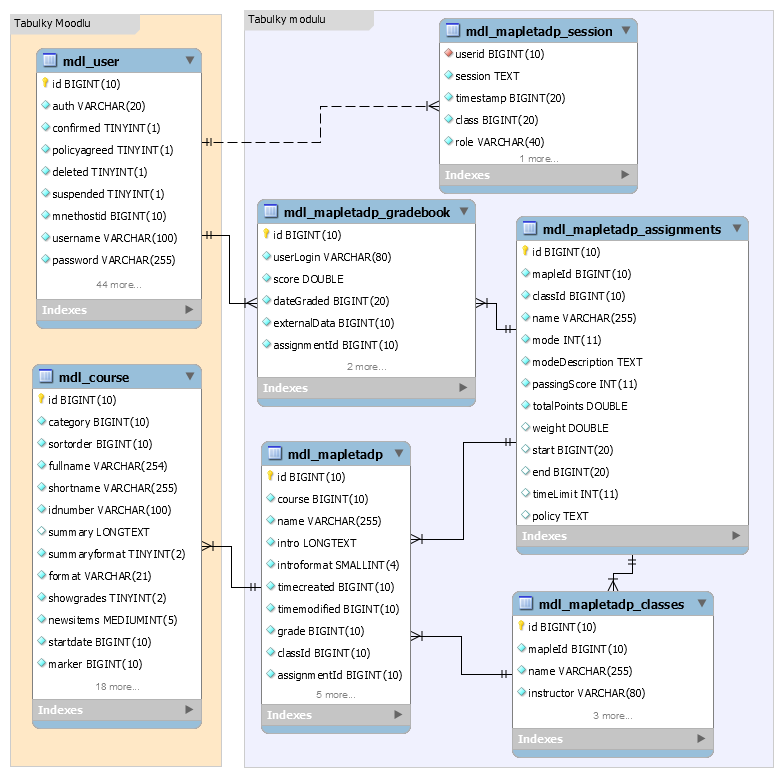
\includegraphics[width=120mm]{images/datamodel.png}
		   \end{center}
		  \caption{Databázový model pro navrhované rozšíření.}
		  \label{fig:datamodel}
		\end{figure}
\subsection*{Tabulka mdl\_mapletadp}
Moodle u~svých rozšíření vyžaduje tabulku pojmenovanou jako prefix mdl\_ a název rozšíření. Tabulka musí obsahovat atributy společné pro všechny výukové moduly. Mimo jiné jsou v~tabulce uchovány atributy specifické pro jednotlivé instance modulu v~kurzech.
\begin{itemize}
	\item \textit{id} -- identifikátor tabulky, Moodle jej vyžaduje u~všech tabulek při práci s~Moodle Data Api 
	\item \textit{course} -- cizí klíč do tabulky mdl\_course (tabulka s~instancemi kurzů), umístění modulu v~instanci kurzu 
	\item \textit{name} -- název modulu v~daném kurzu
	\item \textit{timecreated} -- UNIX časové razítko s~datem a časem vytvoření
	\item \textit{timemodified} -- UNIX časové razítko s~datem a časem poslední změny
	\item \textit{grade} -- 
	\item \textit{classId} -- cizí klíč do tabulky mdl\_mapleta\_classes (ukazuje na atribut mapleId), z~důvodu zachování lokální konzistence
	\item \textit{assignmentId} -- cizí klíč do tabulky mdl\_mapleta\_assignments (ukazuje na atribut mapleId)
\end{itemize}

\subsection*{Tabulka mdl\_mapletadp\_assignments}
V~této tabulce se udržují lokální kopie úkolů ve vazbě na třídu.
\begin{itemize}
	\item \textit{id} -- identifikátor
	\item \textit{mapleId} -- cizí klíč v~systému Maple T.A. pro úkol
	\item \textit{classId} -- cizí klíč v~systému Maple T.A. pro třídu
	\item \textit{name} -  jméno úkolu
	\item \textit{mode} -- typ úkolu
	\item \textit{modeDescription} -- popis typu úkolu
	\item \textit{passingScore} -- minimální hodnota výsledku pro splnění úkolu v~Maple T.A.
	\item \textit{totalPoints} -- maximální hodnota výsledku
	\item \textit{weight} -- váha výsledku z~úkolu
	\item \textit{start} -- datum, odkdy je úkol aktivní
	\item \textit{end} -- datum, dokdy je úkol aktivní
	\item \textit{timeLimit} -- časový limit
	\item \textit{policy} -- seznam politik pro hodnocení
\end{itemize}

\subsection*{Tabulka mdl\_mapletadp\_classes}
Do tabulky mdl\_mapletadp\_classes se ukládají lokální kopie tříd.
\begin{itemize}
	\item \textit{id} -- identifikátor
	\item \textit{mapleId} -- cizí klíč třídy v~systému Maple T.A.
	\item \textit{name} -- jméno třídy
	\item \textit{instructor} -- jméno instruktora
\end{itemize}
\subsection*{Tabulka mdl\_mapletadp\_gradebook}
Do této tabulky se stahují data s~výsledky uživatelů z~jednotlivých úkolů. Data budou nadále zpracovávána a zobrazována v~rozšířeních dle potřeby.
\begin{itemize}
	\item \textit{id} -- identifikátor
	\item \textit{userLogin} -- uživatelské jméno uživatele, který plnil úkol v~systému Maple T.A.
	\item \textit{score} -- počet bodů, které uživatel obdržel
	\item \textit{dateGraded} --  UNIX časové razítko s~datem a časem dokončení (oznámkování)
	\item \textit{externalData} -- identifikátor uživatele, který Moodle předal při spuštění úkolu
	\item \textit{assignmentId} --   cizí klíč do tabulky mdl\_mapleta\_assignments (ukazuje na atribut mapleId)
\end{itemize}

\subsection*{Tabulka mdl\_mapletadp\_session}
Některé z~webových služeb vyžadují pro práci atribut SESSIONID, který slouží jako identifikátor relace uživatele. Aby pro každý jednotlivý požadavek nebylo nutné si tento znovu vyžádat, udržuji si ho v~tabulce ve vazbě na uživatele a kontext. 
\begin{itemize}
	\item \textit{id} -- identifikátor
	\item \textit{userid} -- cizí klíč do tabulky mdl\_users
	\item \textit{session} -- klíč relace SESSIONID
	\item \textit{timestamp} -- časové razítko vytvoření relace
	\item \textit{class} -- identifikátor třídy v~systému Maple T.A., pro který byla vytvořena relace
	\item \textit{role} -- označení uživatelské role v~systému Maple T.A., pro kterou byla vytvořena relace
\end{itemize}
	\section{Struktura modulu a její realizace}
Pro implementaci vlastního konektoru jsem zvolil model o~více vrstvách, kde každá vrstva postupně odbavuje požadavek na data (obrázek \ref{fig:strukturamodulu}).

		\begin{figure}[htb]
		  \begin{center}
		    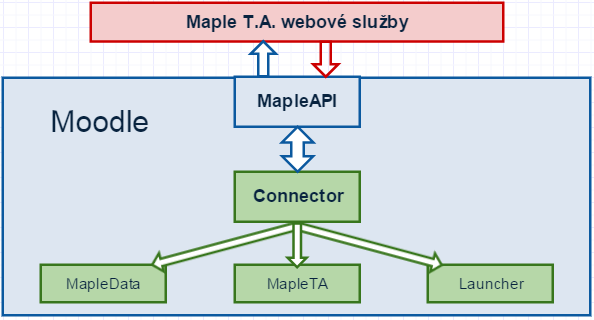
\includegraphics[width=110mm]{images/struktura_modulu.png}
		   \end{center}
		  \caption{Struktura navrhovaného modulu}
		  \label{fig:strukturamodulu}
		\end{figure}
Nejnižší vrstvu tvoří třída MapleAPI, která má na starost vlastní komunikaci s~webovými službami. Mezi hlavní funkce patří funkce call, která pomocí cURL knihovny odesílá POST Request. URL se získává z~nastavení modulu a tělo se skládá z~parametrů, které chodí v~podobě asociativního pole. Klíče pole používají pro vytvoření párových značek XML požadavku, do kterých se poté vkládají hodnoty z~pole:
\begin{lstlisting}[language=PHP, caption=Algoritmus k~převedení asociativního pole na XML]
public function arrayToXML($request) {
  $xml_data = new \SimpleXMLElement('<Request></Request>');
  foreach ($request as $key => $value) {
     if (is_array($value)) {
       if (is_numeric($key)) {
         $key = 'item' . $key;
       }
       $subnode = $xml_data->addChild($key);
        array_to_xml($value, $subnode);
      } else {
         $xml_data->addChild("$key", htmlspecialchars("$value"));
      }
  }
  return $xml_data;
}
\end{lstlisting}

Naopak odpověď získaná v~podobě XML se parsuje na asociativní pole. Zde se využívá následující posloupnosti příkazů:
\begin{lstlisting}[language=PHP, caption=Převedení XML na asociativní pole.]
public function XMLToArray($xmlstring) {
    
  $xml = simplexml_load_string($xmlstring);
  $json = json_encode($xml);
  $array = json_decode($json, TRUE);

   return $array;
}

\end{lstlisting}
 Funkce \texttt{simplexml\_load\_string()} má jako první parametr řetězec, ze kterého se pokouší vytvořit objekt pro knihovnu SimpleXML. Jako řetězec funk\-ci předáme odpověď z~volání webových služeb. Další dvě volání jen využívají vlastnosti převodu objektu nebo pole na objekt JSON a zpět. V~tomto případě se bere objekt vytvořený v~předchozím kroku, vytvoří se JSON voláním funkce \texttt{json\_encode(\$object)}. V~posledním kroku se volá funkce \texttt{json\_decode(\$json, TRUE)}. Druhý atribut nastavený na TRUE určuje za návratovou hodnotu asociativní pole (nastavením na FALSE by se vytvořil objekt).
	

Druhou úroveň modelu tvoří třída Connector, jejíž stavba se blíží návrhovému vzoru \emph{model-view-controller}\footnote{Více na \url{http://blog.codinghorror.com/understanding-model-view-controller/}}. Vrstva data ještě neprezentuje, proto zde chybí část pohledu. Vrstva používá a sbírá parametry do pole pro volání MapleAPI. U~dat provádí kontrolu návratového statusu. Connector také drží konstanty, které se používají k~volání webových služeb (například jména rolí). Jako příklad si uvedeme metodu modelu Connector, která jako vstupní parametry očekává identifikátor třídy a uživatele, nepovinným parametrem je identifikátor úkolu a na jeho základě se vrací úkol (je-li hodnota větší než nula) nebo seznam úkolů dané třídy:
\begin{lstlisting}[language=PHP, caption=Zpracování dat vrácených z Connectoru.]    
public function getAssignments($classID,$user,$assigmentID = 0) {
  $params = $this->getAssignmentsParams($classID, $assigmentID);
   if ($params !== false) {
     $session = $this->getSessionID($user, Connector::MAPLE_ROLE_ADMIN, $classID);
     $response = $this->sendRequest('ws/assignment', $params, $session);
     $dataset = $this->getResponse($response);
      if ($dataset !== false) {
          return $dataset;
      }
  }
  return false;
}

\end{lstlisting}

Na třetí úrovni leží vlastní implemenatace modulu s~kontrolery a moduly, které s~daty a informacemi z~druhé vrstvy pracují. Potřeby této práce naplňují tři částí. První tvoří model \emph{MapleData}, která získává a kontroluje data z~Connectoru, a poté je ukládá, mění, maže, vytváří a vrací z~lokálních tabulek. Druhou částí je \emph{MapleTA}, která má na starost vytvoření instance, zobrazení dat ve formulářích a funkce pro spuštění synchronizace dat a známek. Poslední částí je \emph{Launcher}, který je výchozím bodem pro práci s~automatickým přihlášením a spuštěním specifické části aplikace Maple T.A. (úkol, domácí stránka třídy, administrace systému atd.).

	\section{Detaily implementace}
Uvedeme si příklady implementace vlastního konektoru a vysvětlíme si, jak ovlivňují chování systému.
\subsection{Nastavení modulu po instalaci}
První věcí po instalaci modulu je jeho konfigurace (ta je dostupná i kdykoliv později) pro připojení k~serveru a drobná nastavení chování samotného modulu. K~tomu se využívá souboru \emph{settings.php}, který patří mezi soubory podporované Moodlem jako část rozšíření, a ten zařadí toto nastavení mezi ostatní klasická nastavení (dostupné z~menu \textbf{Správa stránek > Moduly > Moduly činností > Maple T.A.}). Tento tvoří specifický formulář (obrázek \ref{fig:maplesettings}), jehož atributy jsou uloženy mezi nastavení Moodlu, a jsou tedy dostupné odkudkoliv z~celého Moodlu. Mezi zadávané atributy patří:
\begin{itemize}

\item Protokol -- nastavení HTTP nebo HTTPS podle protokolu, na kterém beží server Maple T.A.
\item Jméno server -- URL server s~instalací Maple T.A. včetně portu (je-li používán)
\item Kontext -- část URL, kterou zadáváte při vstupu do Maple T.A. z~webového prohlížeče
\item Sdílené heslo -- slouží k~podepisování komunikace mezi Moodlem a Maple T.A.
\item Životnost SessionID -- nastavení doby, po kterou si Moodle drží identifikátory sezení
\item Pouze uživatelé z~Moodlu -- nastavení zobrazení uživatelů v~Moodlu (všichni uživatelé Maple T.A. nebo pouze ti z~Moodlu); využívá se například v~knize známek
\end{itemize}
		\begin{figure}[htb]
		  \begin{center}
		    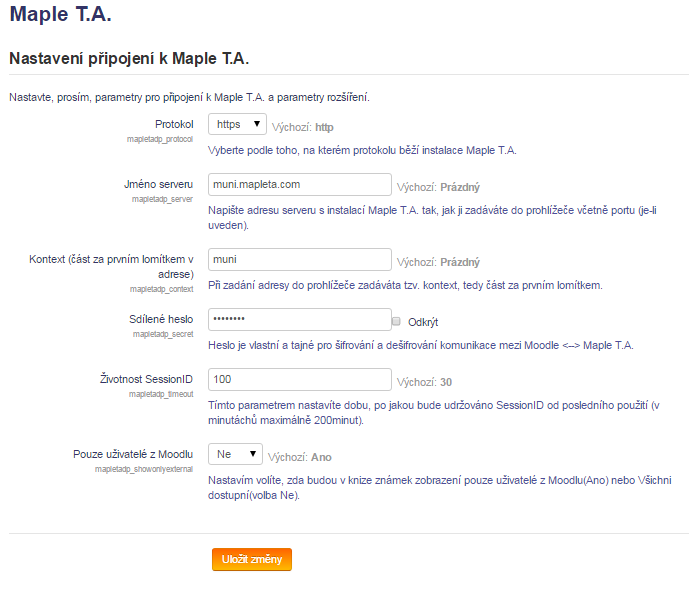
\includegraphics[width=120mm]{images/maple_settings.png}
		   \end{center}
		  \caption{Formulář pro nastavení výukového modulu Maple T.A.}
		  \label{fig:maplesettings}
		\end{figure}

\subsection{Vytvoření nové instance}
Výše je zmíněný problém se závislými poli formuláře a způsob řešení v~konektoru od Maplesoftu. Ve vlastním konektoru je tento problém vyřešen pomocí jQuery, což je JavaScriptová knihovna, která programátorovi umožňuje využítí JavaScriptu jednoduše a \emph{„udělat více s~méně kodém”}\cite{jquery} (volně přeloženo). Formuláři při vytváření předám všechny dostupné úkoly napříč třídami (knihovna pro práci s~formuláři zpracuje u~select boxů pouze s~data při jeho inicializaci) a skript pole po načtení stránky vyprázdní. Při změně výběru třídy si AJAXovým voláním získám úkoly, které k~dané třídě patří:
\begin{lstlisting}[language=Octave, caption=Volání PHP za pomoci AJAXu; získání hodnot pro závislé pole formuláře.]    
$.ajax({
   method: "POST",
   url: "/mod/mapletadp/assignment_list.php?classID=" + $('#id_classId').val()
}).success(function (data) {
   result_obj = $.parseJSON(data);
   var list = "";
   $('#id_assignmentId').empty();
   $.each(result_obj, function (i, val) {
      list += '<option value="' + i + '">' + val + '</option>';
   });
   $('#id_assignmentId').empty().append(list);

});
\end{lstlisting}

		\subsection{Detail modulu a spuštění úkolu}
Náhled modulu tvoří přehled informací o~úkolu, který je s~modulem spárován (typ úkolu, rozmezí, v~němž je aktivní, maximální počet bodů a počet bodů pro splnění atd.). Student zahájí testování kliknutím na odkaz Spustit úkol. Vytvoří se nové okno, ze kterého se automaticky odesílá přes Launcher POST požadavek na přihlášení a spuštění úlohy. V~případě úspěchu dojde k~přesměrování přímo do úkolu. Výsledky uživatelů, kteří se k~úloze přihlašují z~Moodlu, si Maple T.A. ukládá s~uživatelským identifikátorem Moodlu. Díky tomu se dají výsledky využít pro další rozšiřování modulu.

		\subsection{Nová naplánovaná úloha}
V~textu práce se zmiňuji o~naplánovaných úlohách (cron úlohy), které budou využity pro synchronizaci seznamů a dat. Moodle úlohy, které se provádí automaticky, přenáší do systému úloh spouštěných v~pravidelných intervalech na pozadí aplikace. Moodle využívá pouze jeden skript jako skutečnou úlohu běžící v~CRONu (démon, který v~operačním systému spouští příkazy na pozadí), jedná se o~skript \emph{cron.php}. Administrátor serveru při instalaci Moodlu nastaví, aby byl tento skript pouštěn pravidelně v~krátkých intervalech (například každých pět minut). Nad tímto skriptem leží programová část systému. Moodle umožňuje definovat nové úkoly a definovat četnost spouštění. Úlohy se při aktivaci\emph{ cron.php} provolají podle daného nastavení, čímž se snižuje náročnost prováděných operací (není nutné provádět vždy vše). 

Nový úkol v~Moodlu vznikne provedením několika kroků. Prvním je přidání nové třídy, která rozšiřuje třídu \texttt{core{\textbackslash}task{\textbackslash}scheduled\_task} a implementuje metody \texttt{get\_name()} (vrací jméno úlohy) a \texttt{execute()} (obsahuje kód, který je proveden):
\begin{lstlisting}[language=PHP, caption=Implementace třídy je využíta jako naplánovaná úloha.]    
class synchronize extends \core\task\scheduled_task {
  public function get_name() {
     return get_string('synchronization', 'mod_mapletadp');
  }

  public function execute() {
     global $CFG, $DB, $USER;
     $mapletadp = new \mod_mapletadp\controller\Mapleta($DB, $CFG, $USER);
     $mapletadp->refreshAllData();
  }
}
\end{lstlisting}
Ve druhém kroku se provede registrace úlohy do Moodlu pomocí speciálního souboru \emph{tasks.php}, který obsahuje pole se jmény úloh v~rozšíření a jejich nastavením. Soubor musí být umístěn ve složce db a obsahuje pole:
\begin{lstlisting}[language=PHP, caption=Ukázka záznamu pole ze souboru tasks.php]    
$tasks = array(                                                                                                                    
  array(                                                                                                                          
    'classname' => 'mod_mapletadp\task\synchronize',                                                                            
    'blocking' => 0,                                                                                                            
    'minute' => '*',                                                                                                            
    'hour' => '*',                                                                                                              
    'day' => '*',                                                                                                               
    'dayofweek' => '*',                                                                                                         
    'month' => '*'                                                                                                              
  )
);
\end{lstlisting}
Posledním krokem je navýšení verze a její načtení do paměti (soubor version.php). Poté se již úloha zobrazí v~manažeru úloh, kde administrátor může změnit nastavení úlohy nebo ji vypnout.

		\subsection{Lokální rozšíření}
Lokální rozšíření (obrázek \ref{fig:localext} ) nemá přímý vliv na výukový modul a práci studenta nebo učitele s~úkoly. Je to místo, v~němž mají vznikat další funkcionality, které budou instituce schopny využít. V~rámci diplomové práce rozšíření nabízí následující:
\begin{figure}[htb]
		  \begin{center}
		    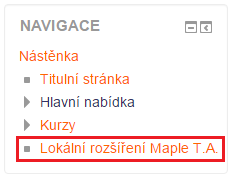
\includegraphics[width=60mm]{images/localext.png}
		   \end{center}
		  \caption{Lokální rozšíření je dostupné z navigace.}
		  \label{fig:localext}
		\end{figure}
\begin{itemize}
 \item Souhrn všech komponent -- nástroj je tvořen jednoduchým skriptem, který ověří funkčnost jednotlivých komponent Maple T.A.(obrázek \ref{fig:monitor}) voláním webových služeb určených pro monitoring. Cílem rozšíření je možnost kontroly systému a zrychlení nalezení problému a případné opravy.
 \item Spustit manuální synchronizaci -- umožňuje spustit ručně skript pro synchronizaci dat a známek. Toho využijete například v~případě, že webhosting poskytuje pouze omezené pouštění CRON skriptů, nebo v~případě, že nastavení administrátorem je nevyhovující a potřebujete okamžitě data k~další práci.
 \item Spustit manuálně CRON úlohu -- je pouhý odkaz na URL, ze které lze spustit CRON úlohy celého Moodlu. Moodle tento odkaz nemá definován a lze pustit pouze zadání URL do prohlížeče.
 \item Kniha známek - tvoří přehled známek z~úkolu v~Maple T.A. s~vazbou na uživatele s~ID v~Moodlu. Pomocí přepínače nastavení připojení k~Maple T.A. se zobrazují výsledky všech studentů nebo jen těch, kteří přistoupili do Maple T.A. z~Moodlu.
\end{itemize}
\begin{figure}[htb]
		  \begin{center}
		    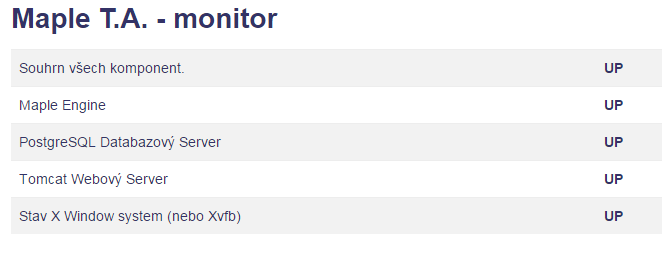
\includegraphics[width=100mm]{images/monitor.png}
		   \end{center}
		  \caption{Monitor komponent systému Maple T.A.}
		  \label{fig:monitor}
		\end{figure}

\chapter{Diskuze}
Během vývoje konektoru jsem se soustředil na funkčnost, kterou doručují i ostatní konektory - přímý přechod z~kurzu na plnění úkolu v~Maple T.A., doplněnou o~jednoduchý monitor dostupnosti komponent. Konektor je plně funkční a je možné jej využít při výuce matematiky, informatiky a případně dalších předmětů, ke kterým učitel využije funkcionality Moodlu (chemie, biologie, fyzika apod.). Funkčnost ovšem prověří až použití v~praxi, stejně jako každý software může obsahovat chyby.

V~návrhu vlastního konektoru jsem připravil některé atributy pro další rozvoj modulu i rozšíření typu local. Ve výukovém modulu se jedná o~možnost využívat příznak dokončení činnosti tak, aby mohl být zapojený do přípravy kurzu s~návaznostmi na další moduly. Společně s~přidáním příznaku dokončení lze přidat i známkování činnosti na základě známek získaných v~Maple T.A. V~tomto případě bude třeba detailnější analýza webové služby vracející hodnocení z~knihy známek, především se zaměřením na návratové hodnoty ve spojitosti s~podmínkami pro splnění kurzu.

Dalším bodem pro rozvoj je využití webových služeb pro automatické odesílání známek z~Maple T.A. do Moodlu a jejich zpracování. K~využití této služby je zapotřebí mít úplná administrátorská práva nad instalací Maple T.A. Nejlépe instalace na vlastním serveru, jelikož nastavení této webové služby a práce s~ní vyžaduje změnu konfiguračních souborů.

Vlastní konektor tak otevírá bránu pro další práci s~daty, které je možné z~Maple T.A. získat, a zajisté by se daly najít i další možnosti pro rozšíření (sada vlastních podmínek pro dokončení a dostupnost modulu kopírující možnosti v~Maple T.A., vytvoření vlastních rolí, doplnění lokálního rozšíření o~formulář k~přidání nové třídy, rozcestník pro přímý přístup do Maple T.A. apod.). Vytvořením základního konektoru bylo splněno zadání, ale také položen stavební kámen rozvoje vlastní integrace mezi systémy Moodle a Maple T.A. s~možností úprav dle požadavků každé konkrétní instituce.

\chapter{Závěr}
Cílem diplomové práce bylo navrhnout a implementovat vlastní řešení integrace systému Maple T.A. do LMS Moodle. V~první části práce jsem definoval základní pojmy spojené s~e-learningem a oba systémy představil, rozebral práci s~nimi a jejich základní stavební kameny. Zmínili jsme, jak systémy přistupují k~řízení oprávnění přístupu ke zdrojům a jak mají definované základní uživatelské role. Dále jsem analyzoval strukturu systému Moodle a možnosti jeho rozšíření obecně a poté jsem rozebral existující řešení pro integraci s~Maple T.A. 

Ve druhé části se práce zaměřila na návrh vlastního způsobu integrace. Podívali jsme se na webové služby a jejich účel. Vytvořil jsem návrh, jak by mělo být rozšíření koncipováno, a porovnal některé detaily s~analýzou ostatních možností integrace. Při návrhu a následné implementaci jsem se snažil co nejvíce přiblížit standardům rozšíření pro Moodle, přesto rozšíření navrhnout co nejobecněji, aby se nemuselo zásadně měnit s~každou verzí.

Příprava diplomové práce mi umožnila blíže se seznámit s~nástrojem Maple T.A. a pochopit, jak s~ním pracovat, prozkoumat možnosti integrace nejen s~Moodlem, ale případně i s~dalšími systémy. Na druhé straně mi implementace nového výukového modulu v~LMS Moodle prohloubila znalosti programování pro Moodle a přinesla nové zkušenosti se správou vlastního prostředí Moodle. Výsledkem práce je funkční konektor pro Moodle, který je možné využít na školách k~rozvoji výuky matematiky, a lokální rozšíření, jež může být dále upravováno ke specifickým účelům každé instituce využívající Moodle a Maple T.A.




\printbibliography[heading=bibintoc]
\makeatletter\thesis@blocks@clear\makeatother
\phantomsection %% Print the index and insert it into the
\addcontentsline{toc}{chapter}{\indexname} %% table of contents.

\makeatletter\thesis@blocks@clear\makeatother

\renewcommand{\theHchapter}{A\arabic{chapter}}
\listoffigures
\listoftables
\lstlistoflistings




\appendix %% and start the appendices.

\chapter{Demoverze}
Pro úkázky implementace bez nutnosti nové instalace LMS Moodle a administračních zásahů do testovací instalace Maple T.A. je vytvořena demoverze dostupná na adrese \url{http://fryval.cz/}. V systému jsou připraveni následující uživatele:
\begin{itemize}
\item \textbf{uživatel v roli administrátor}
	\begin{itemize}
		\item Přihlašovací jméno -- admin
		\item Heslo -- na vyžádání
	\end{itemize}
\item \textbf{uživatel v roli učitel}
	\begin{itemize}
		\item Přihlašovací jméno -- ucitel
		\item Heslo -- na vyžádání
	\end{itemize}
\item \textbf{uživatel v roli student}
	\begin{itemize}
		\item Přihlašovací jméno -- student
		\item Heslo -- na vyžádání
	\end{itemize}
\end{itemize}


Instalace má několik omezení:
\begin{itemize}
	\item Sdílené heslo není nastavitelné pomocí nastavení modulu, z důvodu bezpečnosti (pro případ úniku administrátorského hesla) je přímo ve zdrojovém kódu.
	\item Integrace do systému LMS Moodle je provedena z cloudové instalace Maple T.A. dostupné z adresy \url{https://muni.mapleta.com/muni/}.

	\item Webhosting umožňuje nastavit spuštění CRON úlohy pouze 1x za hodinu. Využijte proto pro zrychlení možnosti ručního spuštění naplánovaných úloh z lokálního rozšíření Maple T.A.
	\item Hesla k uživatelským účtům budou zaslána po odevzdání práce vedoucímu a oponentovi, a poté kdykoliv po domluvě. Toto opatření slouží proti poškození systému LMS Moodle, protože jak text, tak instalace jsou veřejně dostupné.
	\end{itemize}

\chapter{Přiložená data}
Následující data jsou součástí diplomové práce:
\begin{itemize}
\item text diplomové práce ve formátu PDF a \LaTeX
\item obrázky použíté v textu práce
\item dokumentace webových služeb Maple T.A. ve formátu PDF
\item ZIP archív zdrojových kódů
\end{itemize}

\end{document}
